\documentclass[8pt,mathserif]{beamer}
\usepackage{amsmath,amssymb,amsthm,graphicx,hyperref,srcltx,changepage}
\usepackage{ctex}



\usepackage{beamerthemetree}%,beamerthemeshadow}
\usepackage{overpic}
\usepackage{color}
\usepackage{multirow}
\usepackage{ltxtable}
\usepackage{hyperref}
\usepackage[hang]{subfigure}
\usepackage[mathscr]{euscript}
\usepackage{bm}

\usefonttheme[onlymath]{serif}
%\usepackage{beamerthemeshadow}
\setbeamertemplate{bibliography item}[text]

\usetheme{Madrid}
%\usetheme{Boadilla}
\newtheorem{property}{Property}

\newcommand\bbR{\mathbb{R}}
\newcommand\bbN{\mathbb{N}}
\newcommand\bxi{\boldsymbol{\xi}}
\newcommand\bx{\boldsymbol{x}}
\newcommand\bq{\boldsymbol{q}}
\newcommand\bu{\boldsymbol{u}}
\newcommand\be{\boldsymbol{e}}
\newcommand\bg{\boldsymbol{g}}
\newcommand\bh{\boldsymbol{h}}
\newcommand\bn{\boldsymbol{n}}
\newcommand\br{\boldsymbol{r}}
\newcommand\bz{\boldsymbol{z}}
\newcommand\bdeta{\boldsymbol{\eta}}
\newcommand\htheta{\hat{\theta}}
\newcommand\bTheta{\boldsymbol{\Theta}}
\newcommand\balpha{\boldsymbol{\alpha}}
\newcommand\brho{\boldsymbol{\rho}}
\newcommand\bPhi{\boldsymbol{\Phi}}
\newcommand\dd{\,\mathrm{d}}
\newcommand\Kn{\mathit{Kn}}
\newcommand\bw{\boldsymbol{w}}
\newcommand\RM{{\cal R}_M}
\newcommand\bdelta{\boldsymbol{\delta}}
\newcommand\cS{{\cal{S}}}
\newcommand\rC[2]{{\rm{C}}_{{#1},{#2}}}
\newcommand\rmC{{\rm{C}}}

\newcommand\bAM{{{\bf{A}}_M}}
\newcommand\bhAM{{\hat{\bf{A}}_M}}
\newcommand\btAM{{\tilde{\bf{A}}_M}}

\newcommand\mN{{\mathcal N}_{D}}
\newcommand\mM{{\mathcal M}}

\newcommand\Rxx{R$xx$~}
\newcommand\NRxx{NR$xx$~}
\newcommand\pdd[1]{\dfrac{\partial}{\partial {#1}}}
\newcommand\pd[2]{\dfrac{\partial {#1}}{\partial {#2}}}
\newcommand\od[2]{\dfrac{\mathrm{d} {#1}}{\mathrm{d} {#2}}}
\newcommand\seq[2]{{{#1}:{#2}}}
%\newcommand\bm[1]{\boldsymbol{#1}}
\newcommand\comment[1]{}


\newcommand\bbC{\mathbb{C}}
\newcommand\bbG{\mathbb{G}}
\newcommand\ba{\bm{a}}
\newcommand\bb{\bm{b}}
\newcommand\bk{\bm{k}}
\newcommand\bt{\bm{t}}
\newcommand\bzero{{0}}
\newcommand\bA{ {\bf A}}
\newcommand\bB{ {\bf B}}
\newcommand\bC{ {\bf C}}
\newcommand\bD{ {\bf D}}
\newcommand\bE{ {\bf E}}
\newcommand\bF{ {\bf F}}
\newcommand\bG{ {\bf G}}
\newcommand\bH{ {\bf H}}
\newcommand\bI{ {\bf I}}
\newcommand\bJ{ {\bf J}}
\newcommand\bK{ {\bf K}}
\newcommand\bL{ {\bf L}}
\newcommand\bM{ {\bf M}}
\newcommand\bN{ {\bf N}}
\newcommand\bO{ {\bf O}}
\newcommand\bP{ {\bf P}}
\newcommand\bPb{{{\bf P}_b}}
\newcommand\bPp{{{\bf P}_p}}
\newcommand\bQ{ {\bf Q}}
\newcommand\bR{ {\bf R}}
\newcommand\bS{ {\boldsymbol{S}}}
\newcommand\bT{ {\bf T}}
\newcommand\bU{ {\boldsymbol{U}}}
\newcommand\bV{ {\boldsymbol{V}}}
\newcommand\bW{ {\bf W}}
\newcommand\bX{ {\bf X}}
\newcommand\bY{ {\bf Y}}
\newcommand\bZ{ {\bf Z}}
\newcommand\bv{\bm{v}}
\newcommand\bbeta{\beta}
\newcommand\bLambda{{\bf \Lambda}}

\newcommand\imag{\boldsymbol{\mathrm{i}}}
\newcommand\mE{{\mathcal{E}}}

\newcommand\He{\text{He}}
\newcommand\Healphau{\text{He}_{\balpha}^{[\bu,\theta]}}
\newcommand\Healpha{\text{He}_{\balpha}}
\newcommand\Hebeta{\text{He}_{\bbeta}}
\newcommand\hatHealphau{\widehat{\text{He}}_{\bm{\alpha}}^{[\bu,\theta]}}
\newcommand\hatHebetau{\widehat{\text{He}}_{\bm{\beta}}^{[\bu,\theta]}}
\newcommand\Halphau{\mathcal{H}_{\balpha}^{[\bu,\theta]}}
\newcommand\Hbetau{\mathcal{H}_{\bbeta}^{[\bu,\theta]}}
\newcommand\Hgammau{\mathcal{H}_{\gamma}^{[\bu,\theta]}}
\newcommand\hatHalphau{\widehat{\mathcal{H}}_{\balpha}^{[\bu,\theta]}}
\newcommand\hatHbetau{\widehat{\mathcal{H}}_{\bbeta}^{[\bu,\theta]}}
\newcommand\Hebetau{\text{He}_{\bbeta}^{[\bu,\theta]}}

\newcommand\bmH{\boldsymbol{\mathcal{H}}^{[u,\theta]}}
\newcommand\bbH{\mathbb H}
\newcommand\mbH{\mathcal{H}^{[\bu, \theta]}}
\newcommand\mHT{\mathcal{H}^{[\bu, \Theta]}}
\newcommand\mH{\mathcal{H}^{[u, \theta]}}
\newcommand\rmspan{\mathrm{span}}

\newcommand\omegau{\omega^{[\bm{u},\theta]}}

\newcommand\bNRxx{\texorpdfstring{{\bf NR}$\boldsymbol{xx}$}{NR$xx$}}

\newcommand\diag{\mathrm{diag}}
\newcommand\tr{\mathrm{tr}}
%\newcommand\note[2]{{{\bf #1}\color{red} [ {\it #2} ]}}
\graphicspath{{images/}}
\DeclareGraphicsRule{*}{pdf}{*}{}
% \DeclareGraphicsRule{.eps}{pdf}{.pdf}{`pstopdf #1`}

{\theoremstyle{remark} \newtheorem{remark}{Remark}}
\newtheorem{proposition}{Proposition}

\AtBeginSection[]
{
  \begin{frame}<beamer>{Outline}
    \tableofcontents[currentsection,hideallsubsections]
  \end{frame}
}

\begin{document}

\title[]{
{
有限体积格式求解偏微分方程的数值实践
}
}

\author[郑灵超]{
  \normalsize  郑灵超}
\institute[]{\normalsize 北京大学数学科学学院}

\date[\today]{\today}


\frame{\titlepage}



\begin{frame}
  \frametitle{有限体积格式}

\end{frame}

\begin{frame}
  \frametitle{数值通量}
\end{frame}


\begin{frame}
  \frametitle{斜率限制器}
\end{frame}


\begin{frame}
  \frametitle{数值算例:线性对流方程} 
    \begin{equation*}
      u_t+u_x = 0 , \quad -1\leq x < 1
    \end{equation*}
    \begin{figure}[H]
        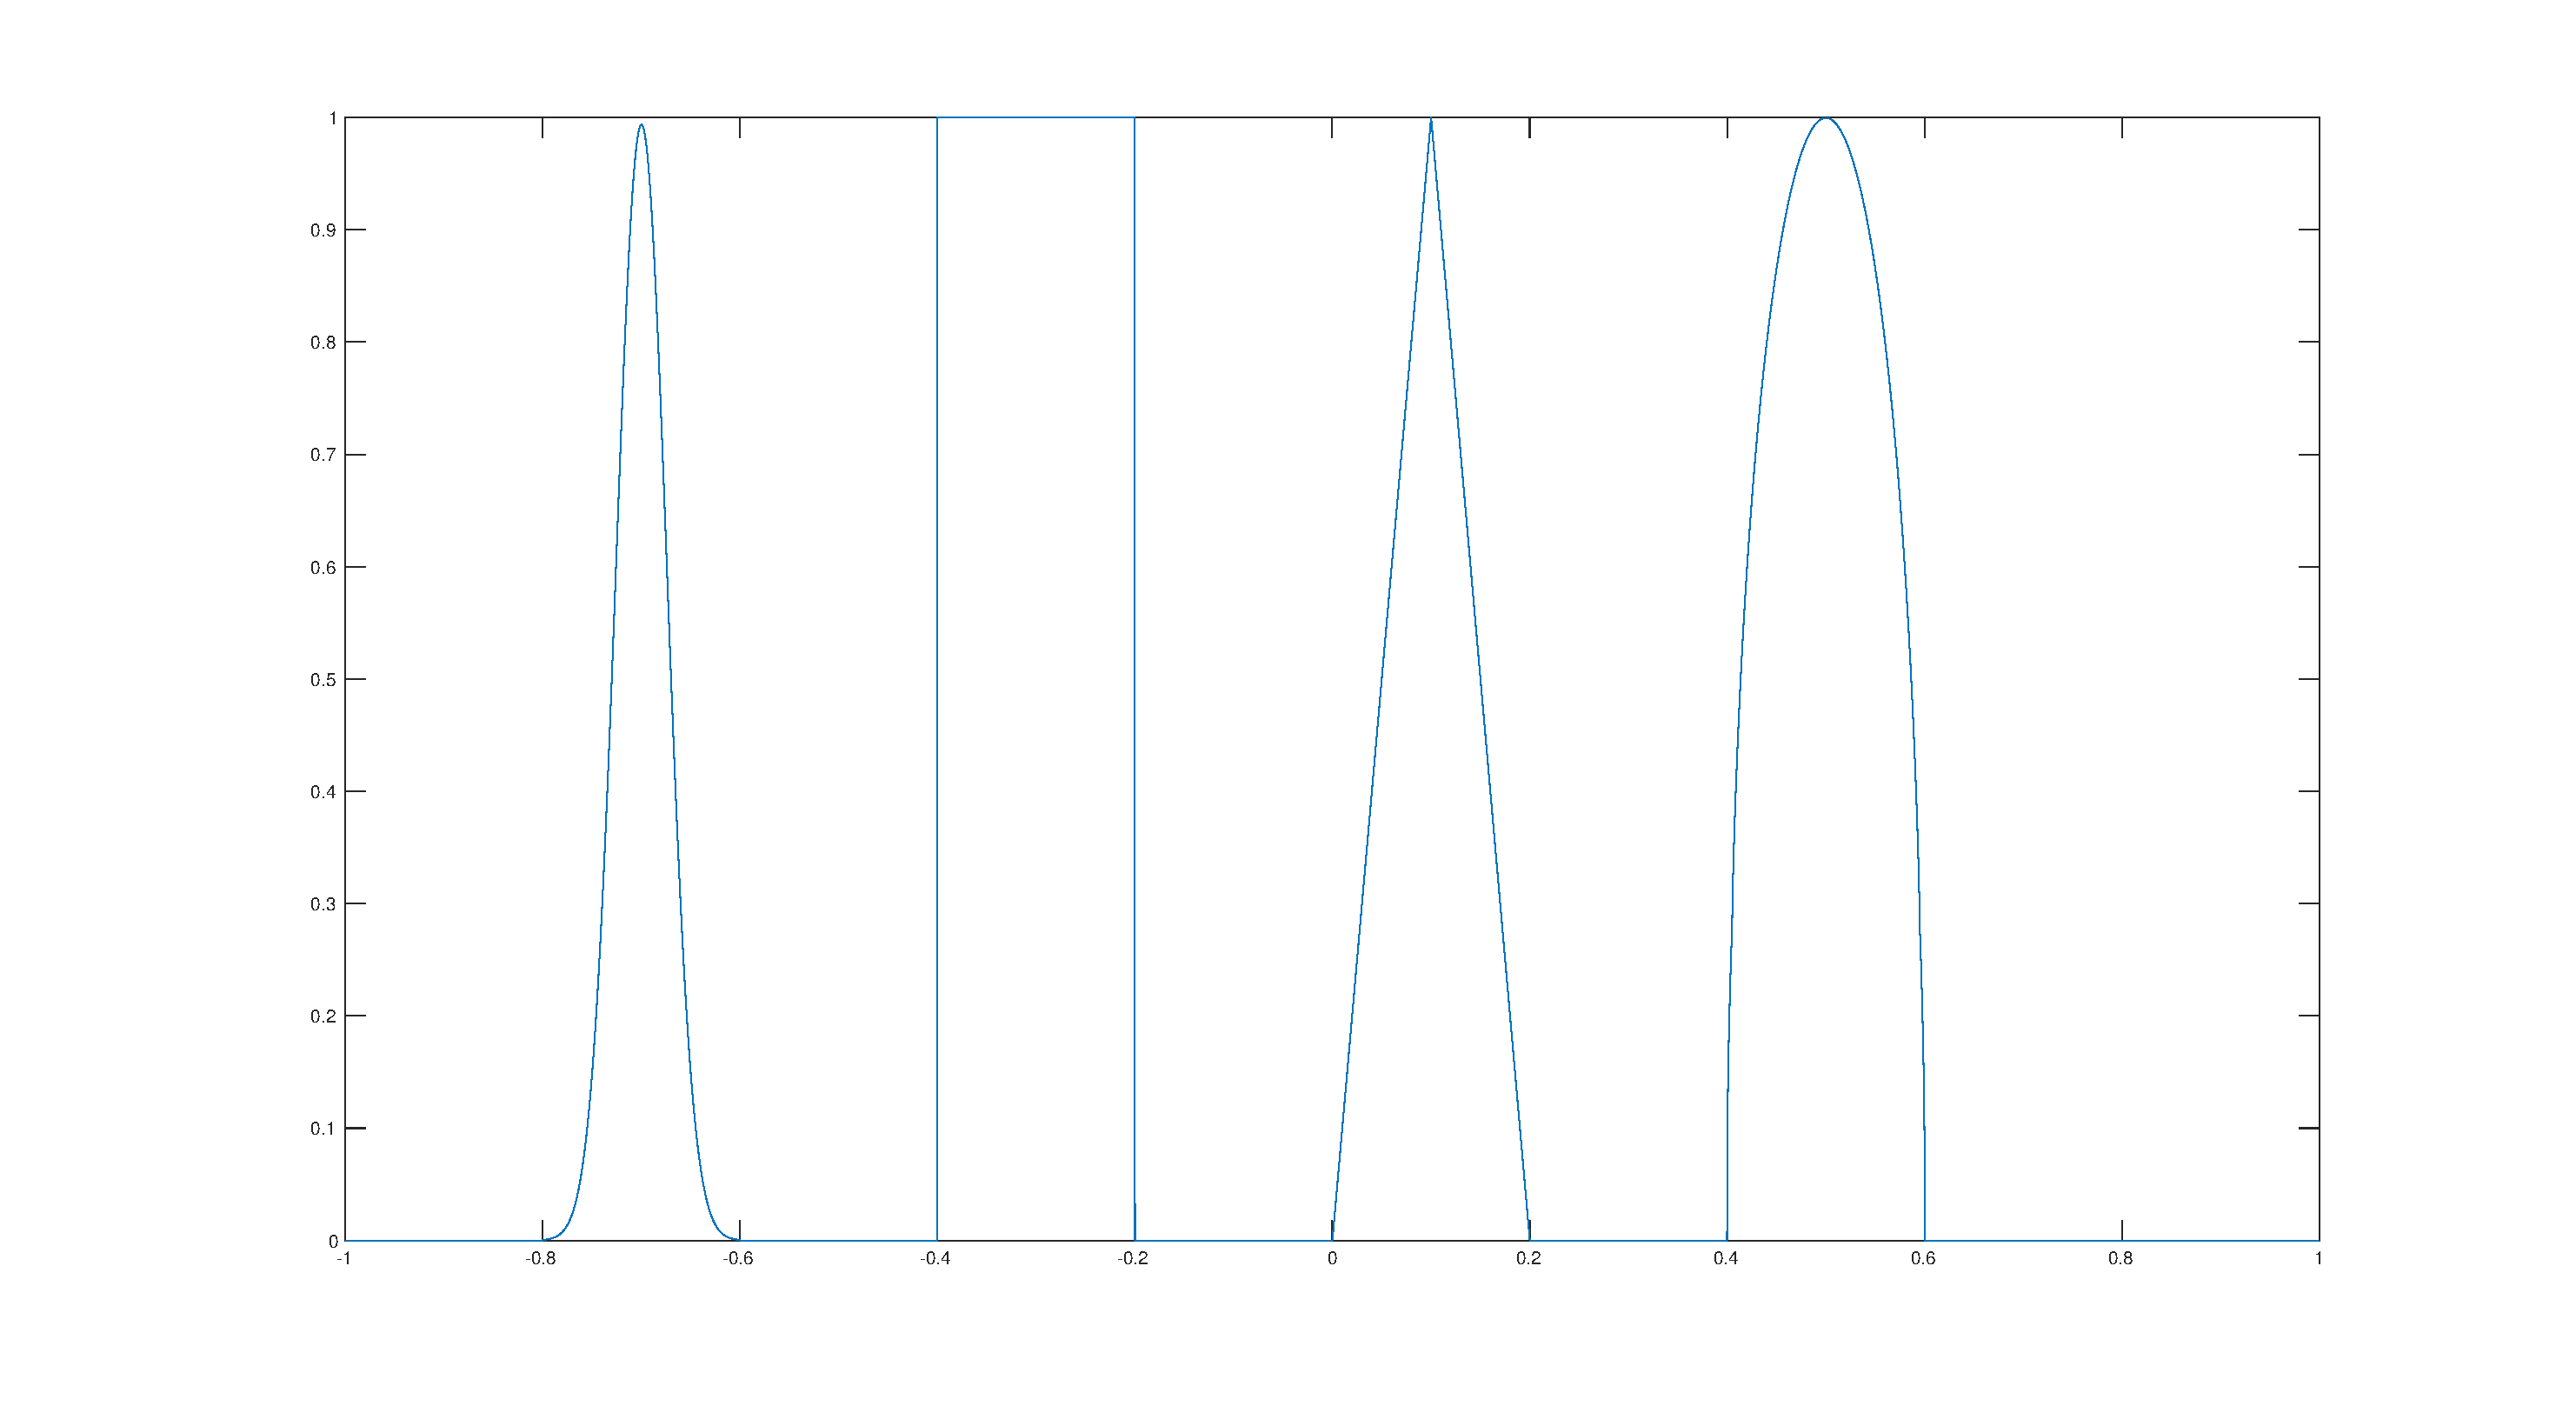
\includegraphics[width=0.45\textwidth]{../doc/images/advection_t0.eps}
      \caption{初始值}
    \end{figure}
\end{frame}
\begin{frame}
  $\qquad t=8, N=10000, CFL=0.6$
  \frametitle{数值算例:线性对流方程}
  \begin{figure}[H]
    \subfigure[LF]{
    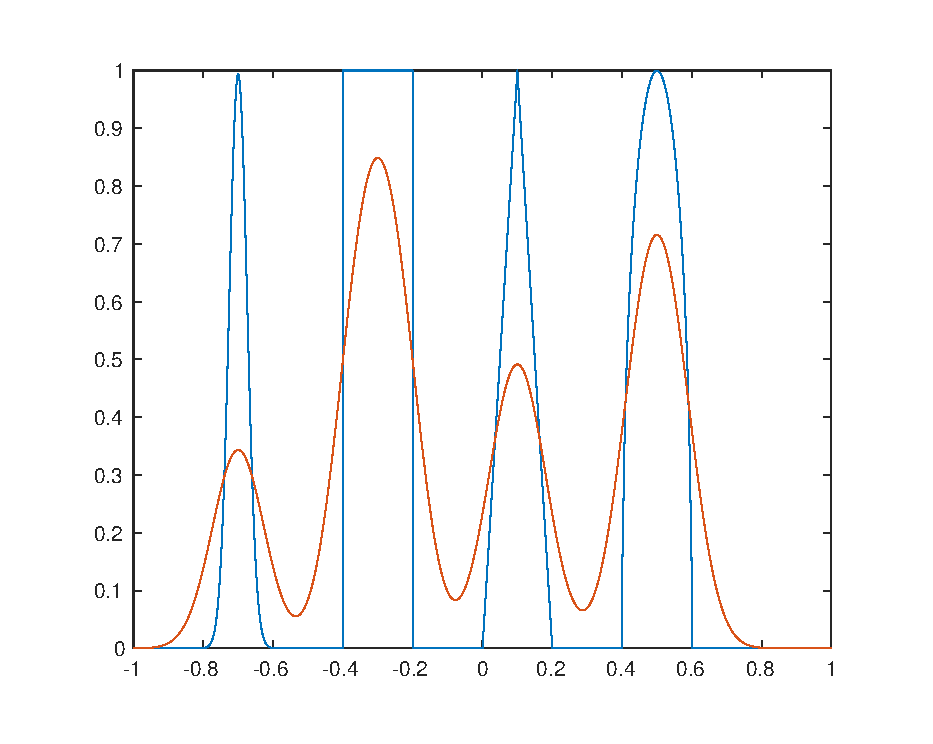
\includegraphics[width=0.23\textwidth,height=0.2\textheight]{../doc/images/advection_LF.eps}}
    \subfigure[LW]{
    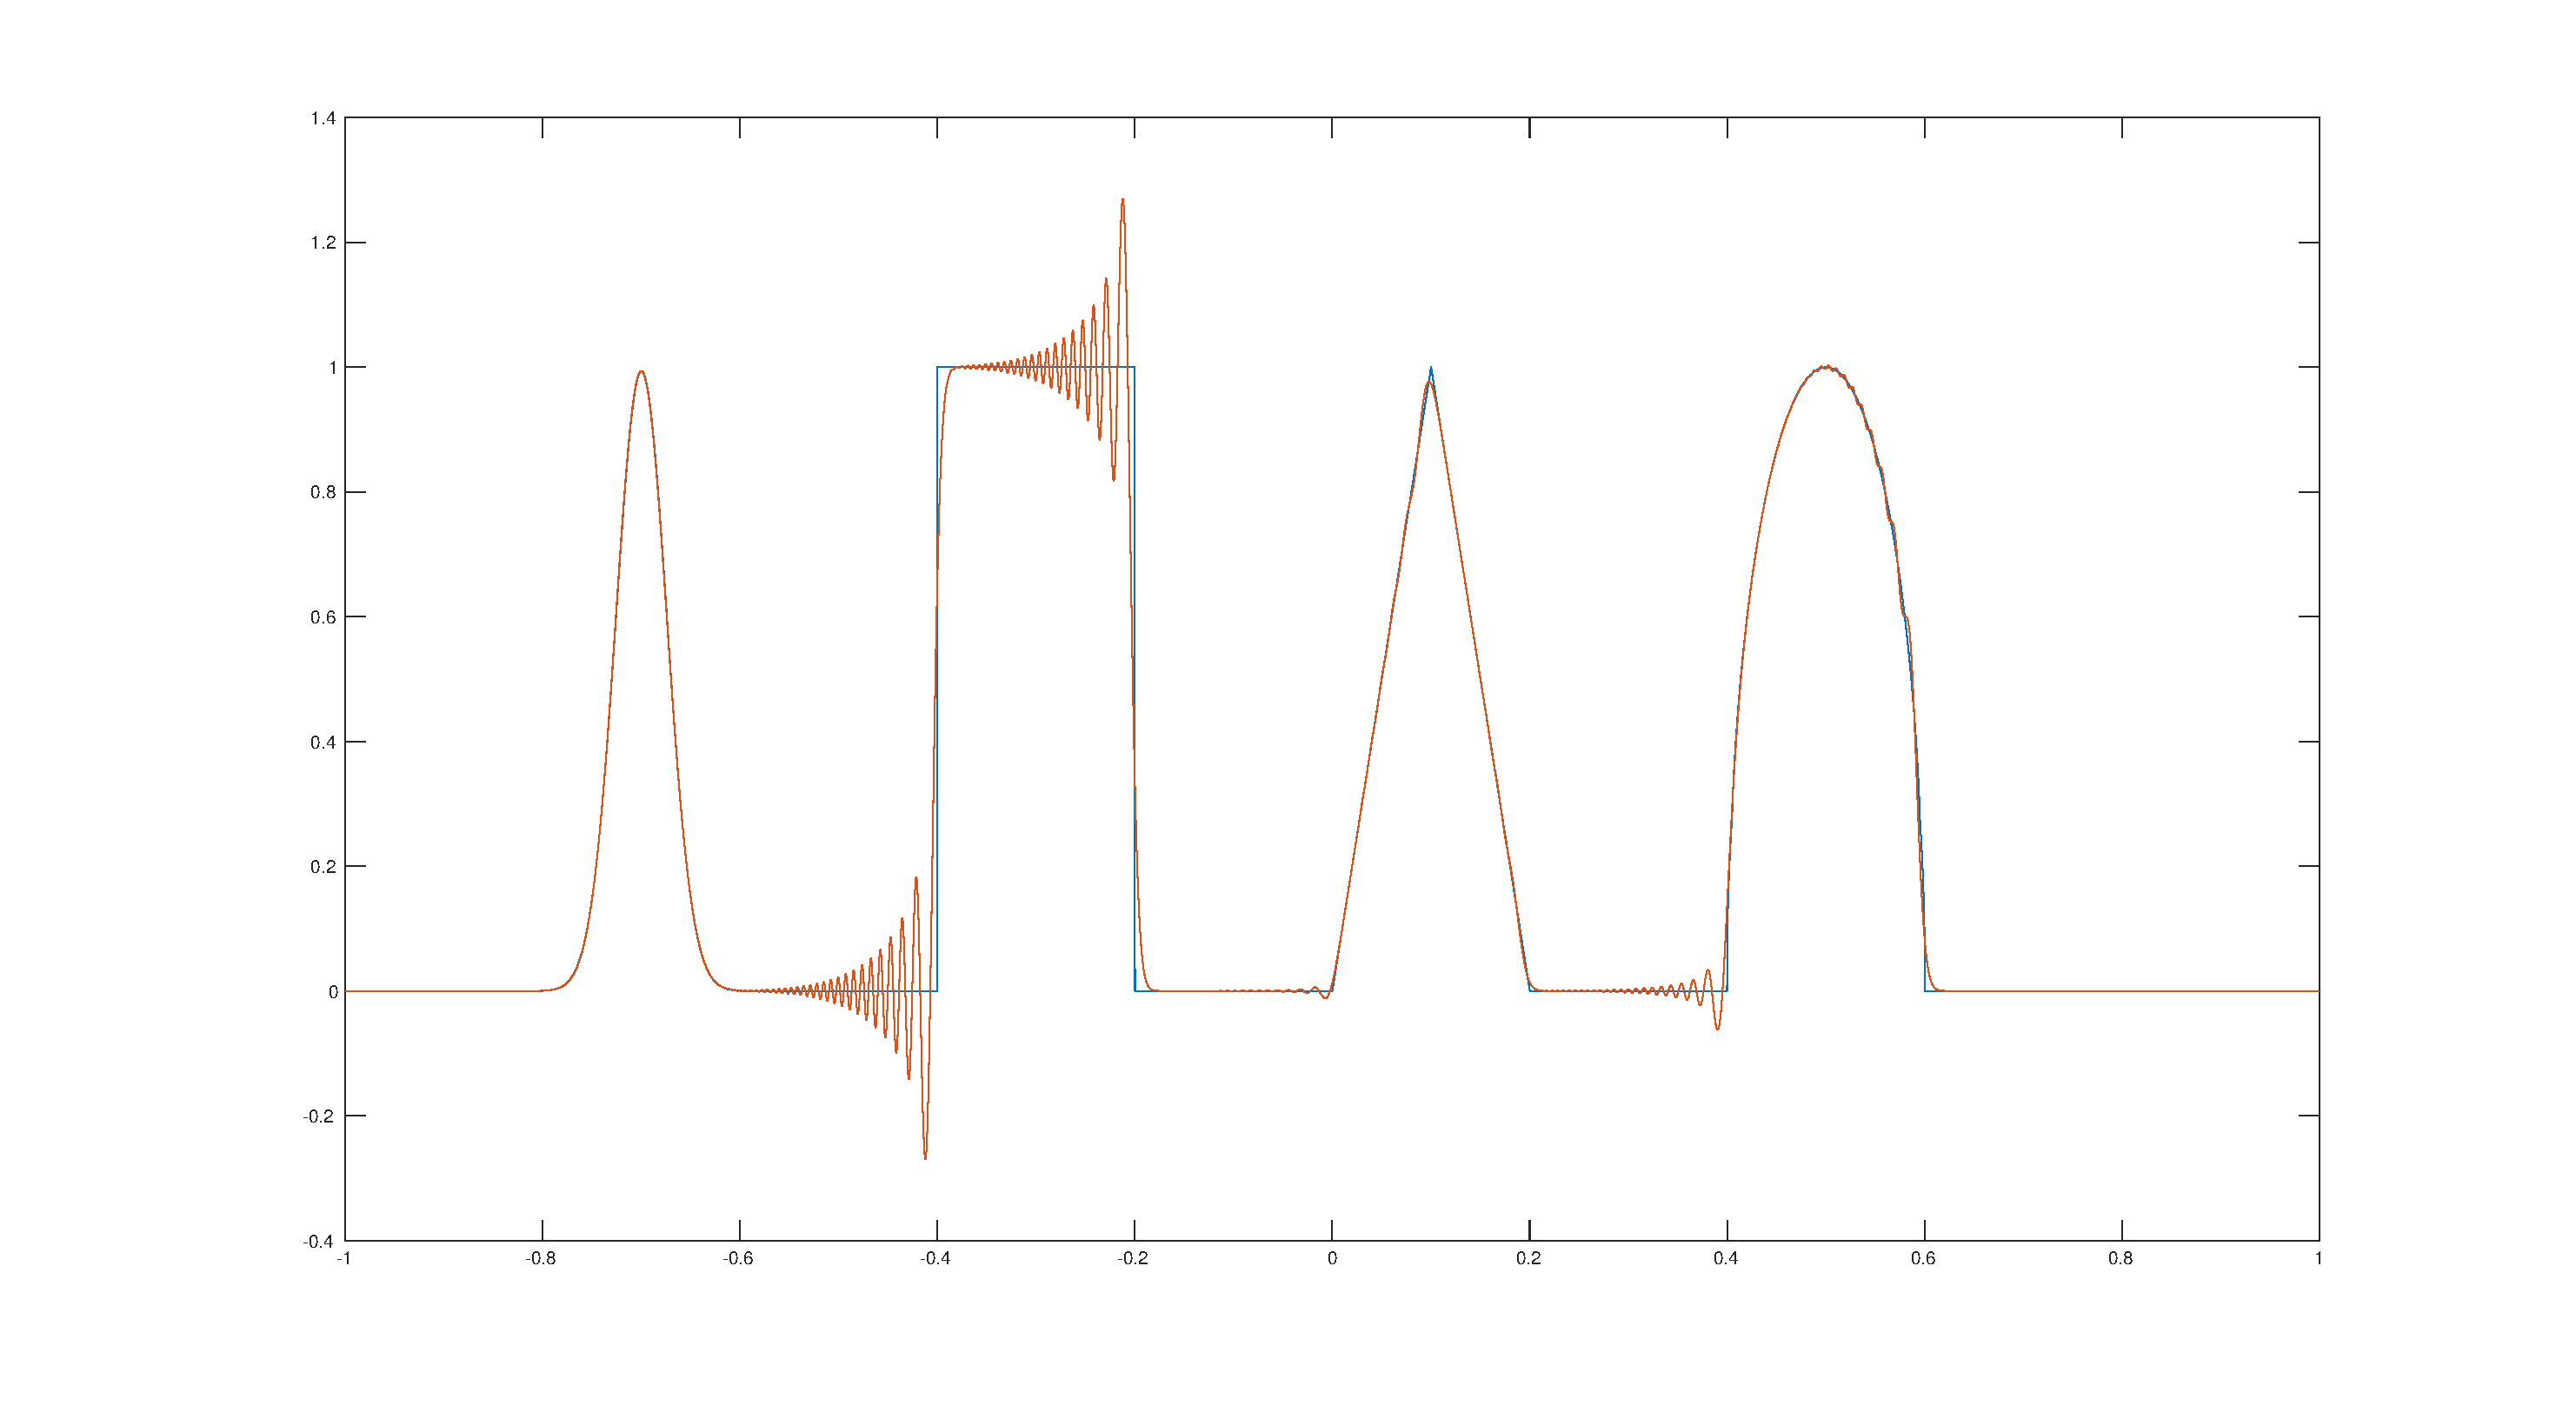
\includegraphics[width=0.23\textwidth,height=0.2\textheight]{../doc/images/advection_LW.eps}}
    \subfigure[Force]{
    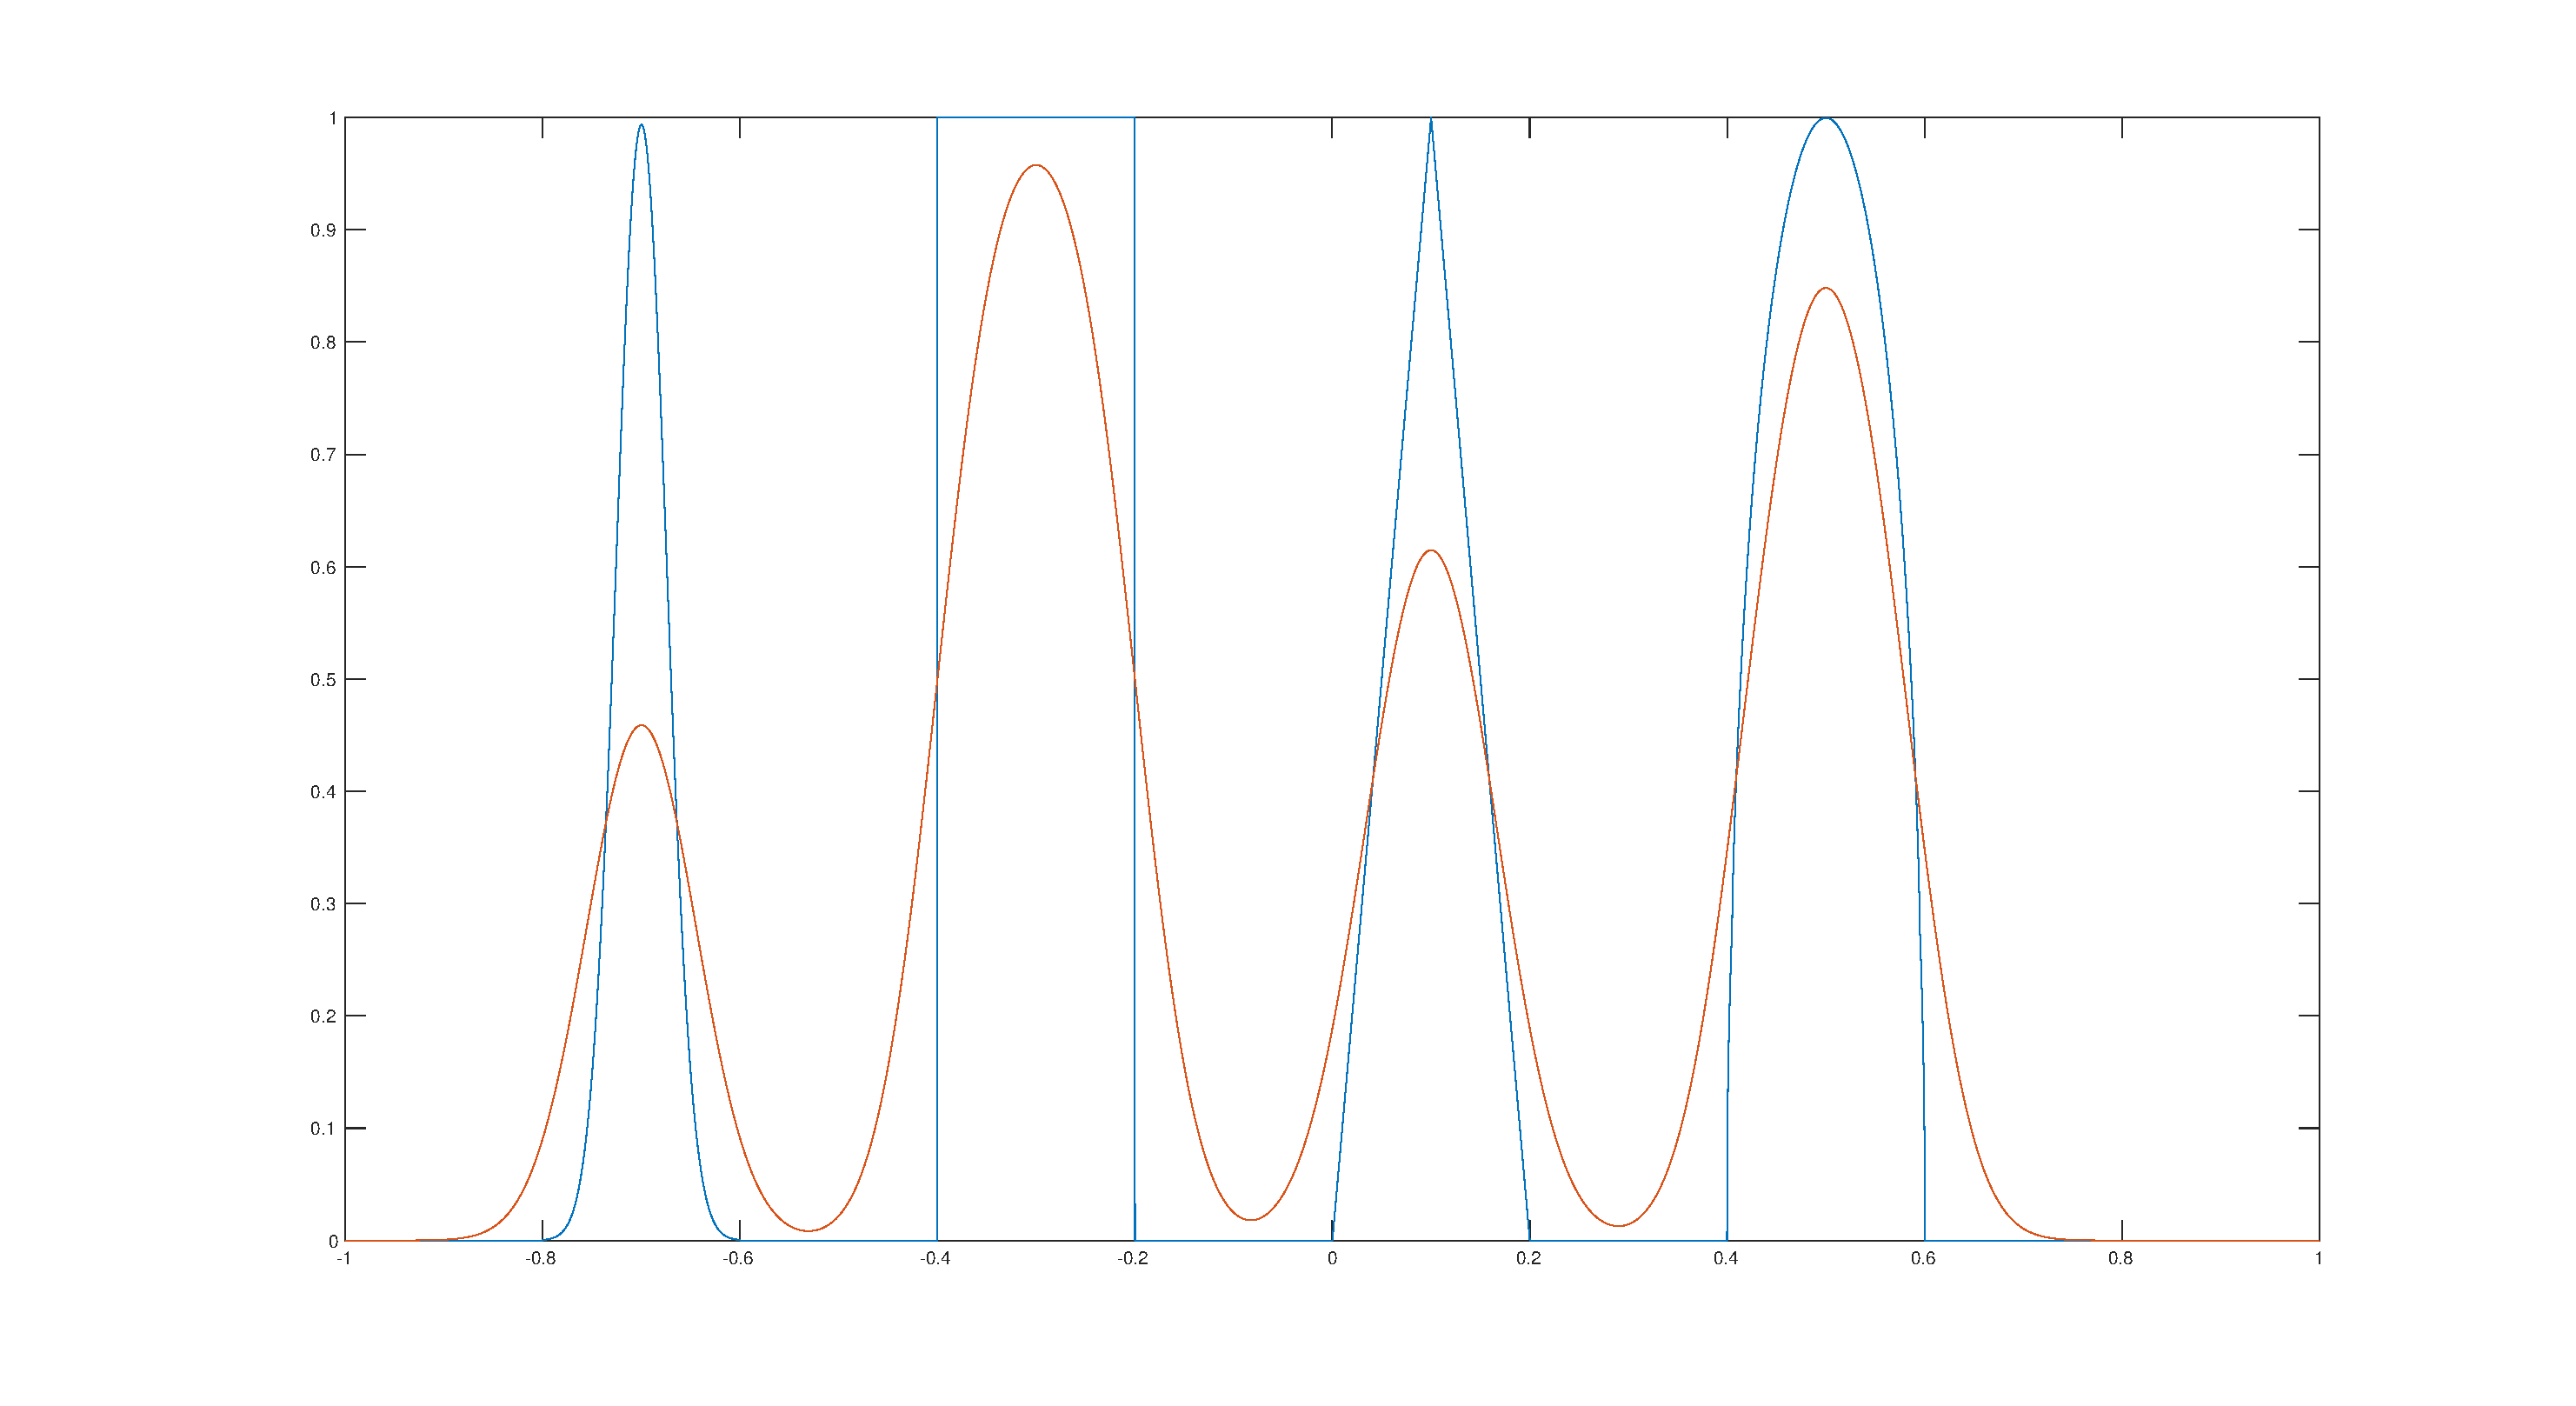
\includegraphics[width=0.23\textwidth,height=0.2\textheight]{../doc/images/advection_Force.eps}}
    \subfigure[Godunov]{
    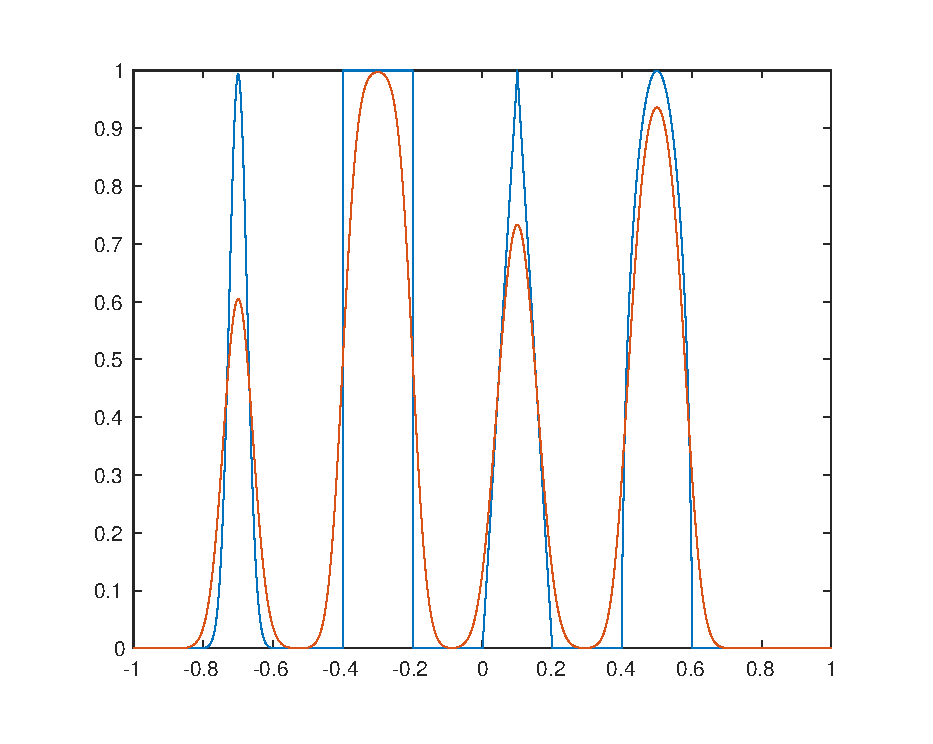
\includegraphics[width=0.23\textwidth,height=0.2\textheight]{../doc/images/advection_Godunov.eps}}
  \end{figure}
  \begin{itemize}
    \item LF格式不会出现震荡,但耗散比较严重。
    \item LW格式没有耗散,但数值震荡现象明显。
    \item Force格式耗散比LF格式略小。
    \item Godunov格式耗散比Force格式小,但还是不能令人满意。
  \end{itemize}
\end{frame}
\begin{frame}
  \begin{figure}[H]
    \subfigure[minmod]{
    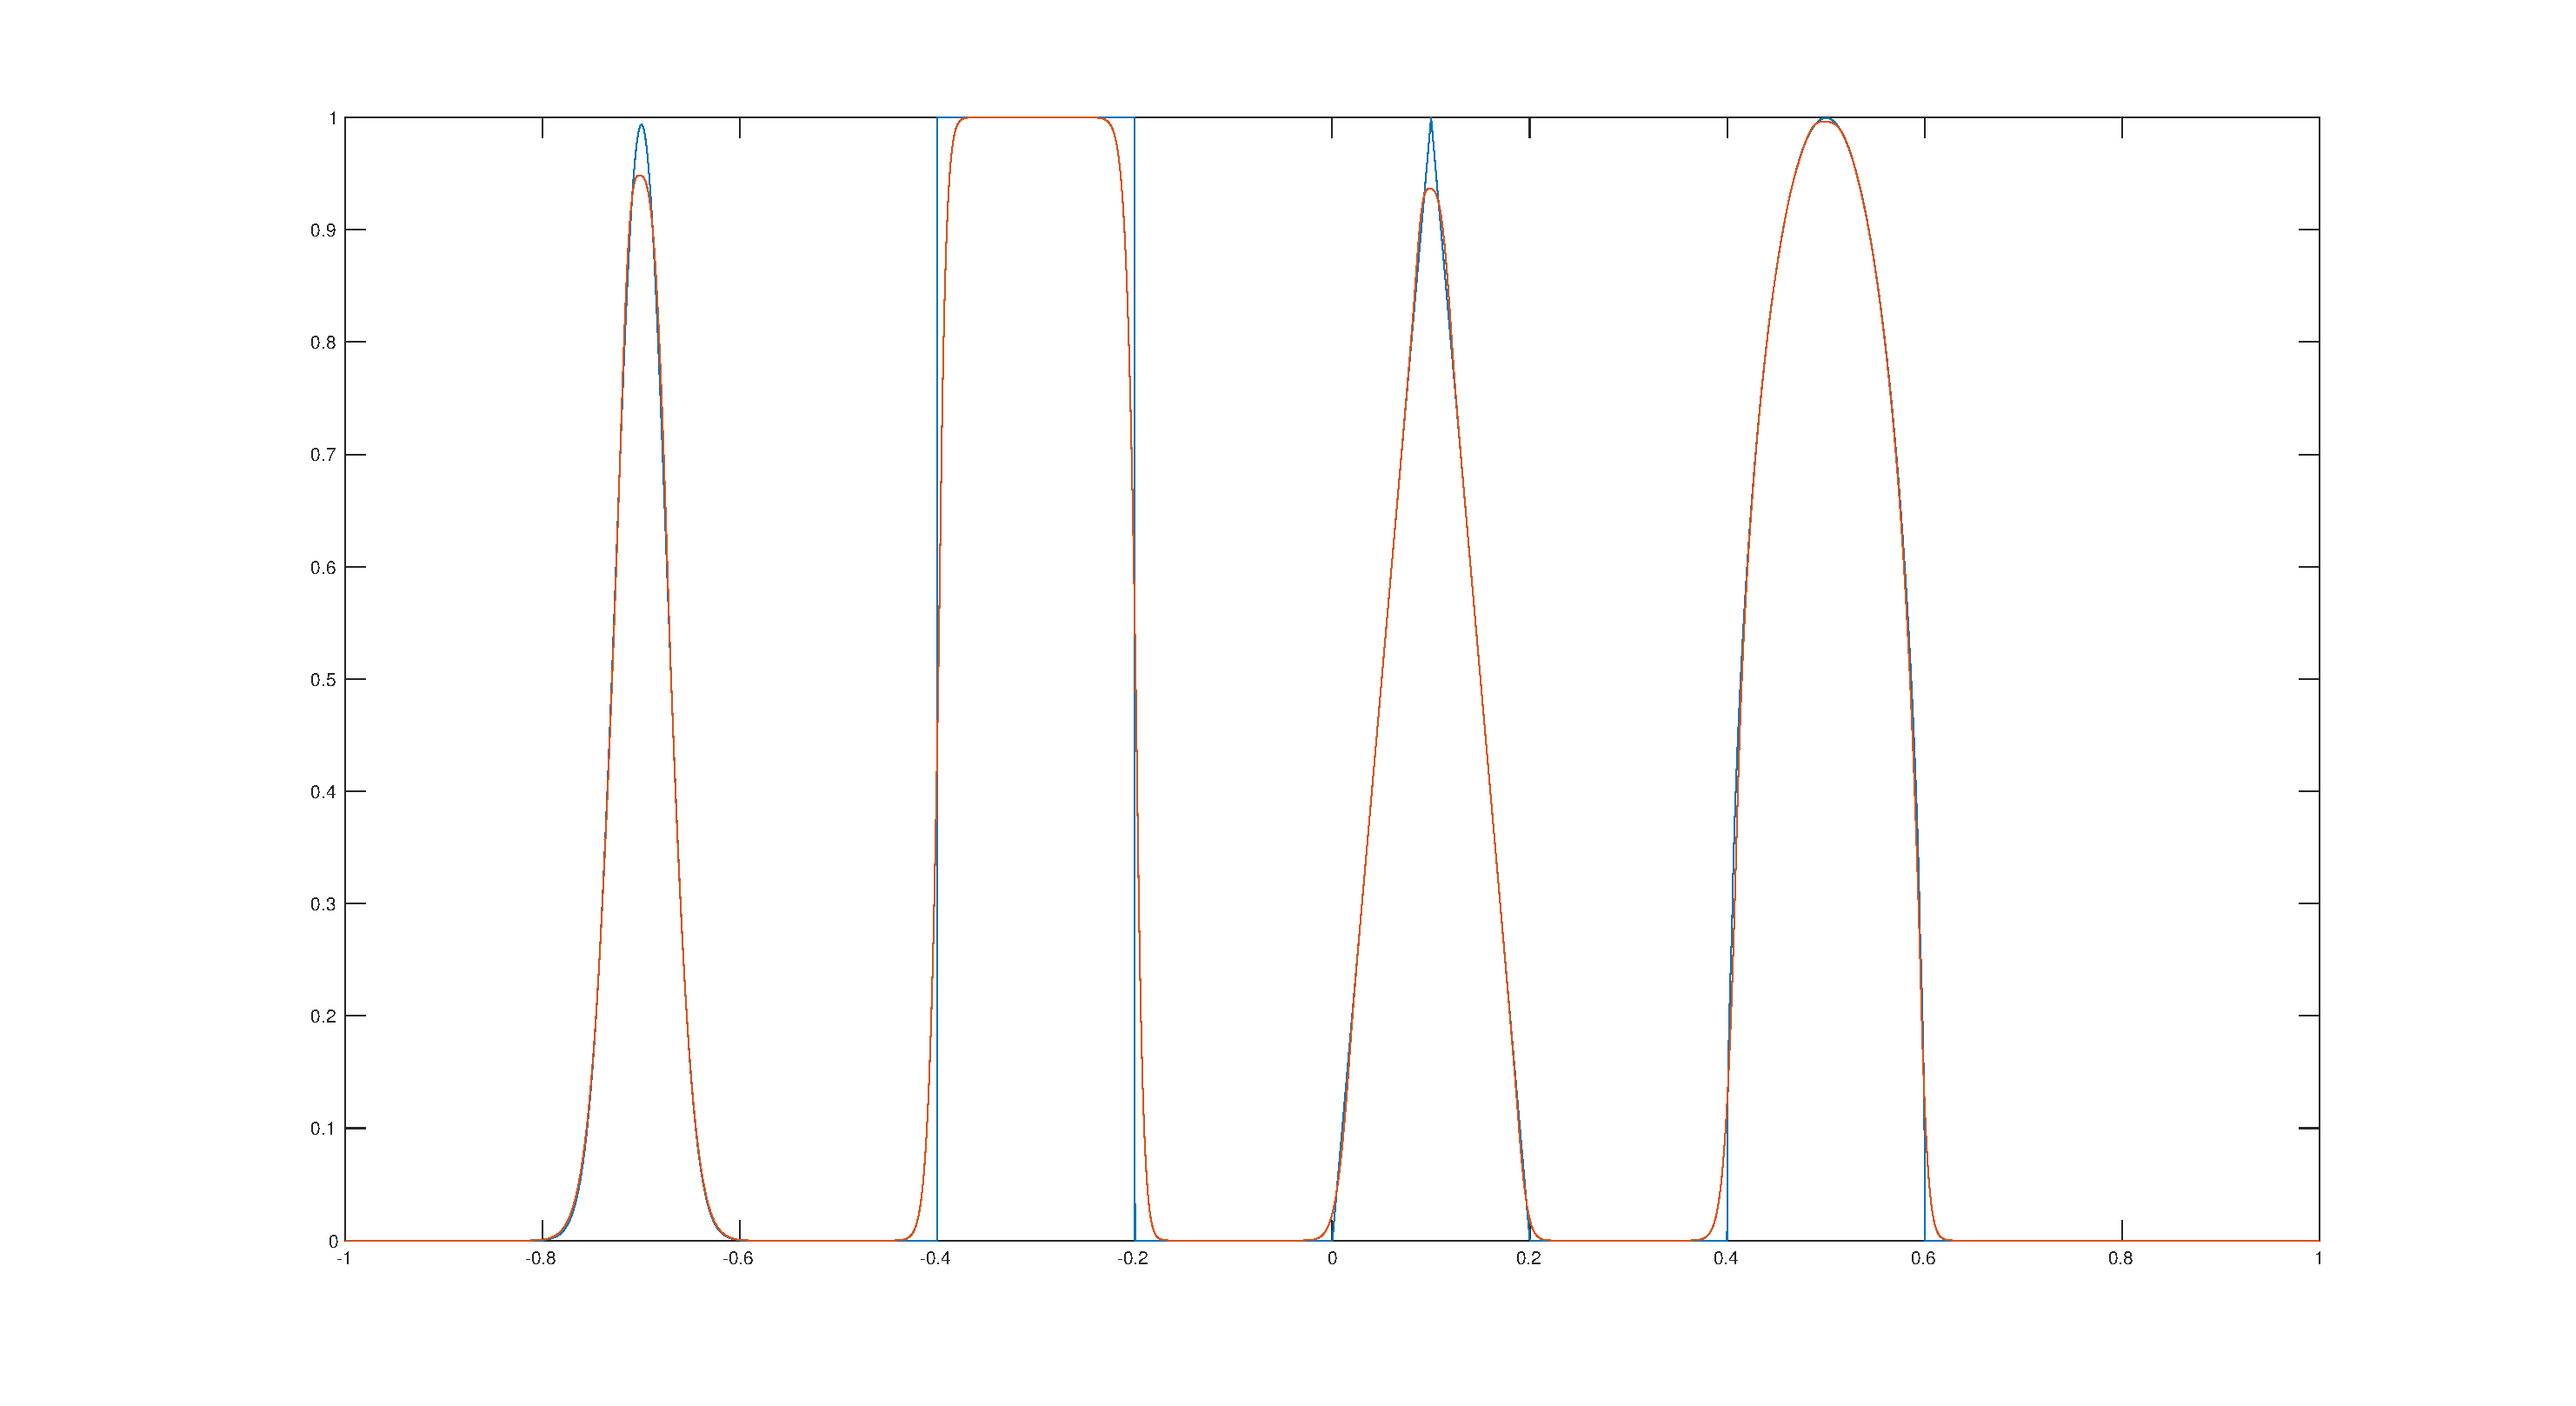
\includegraphics[width=0.45\textwidth,height=0.4\textheight]{../doc/images/advection_LF_minmod_RK3.eps}}
    \subfigure[superbee]{
    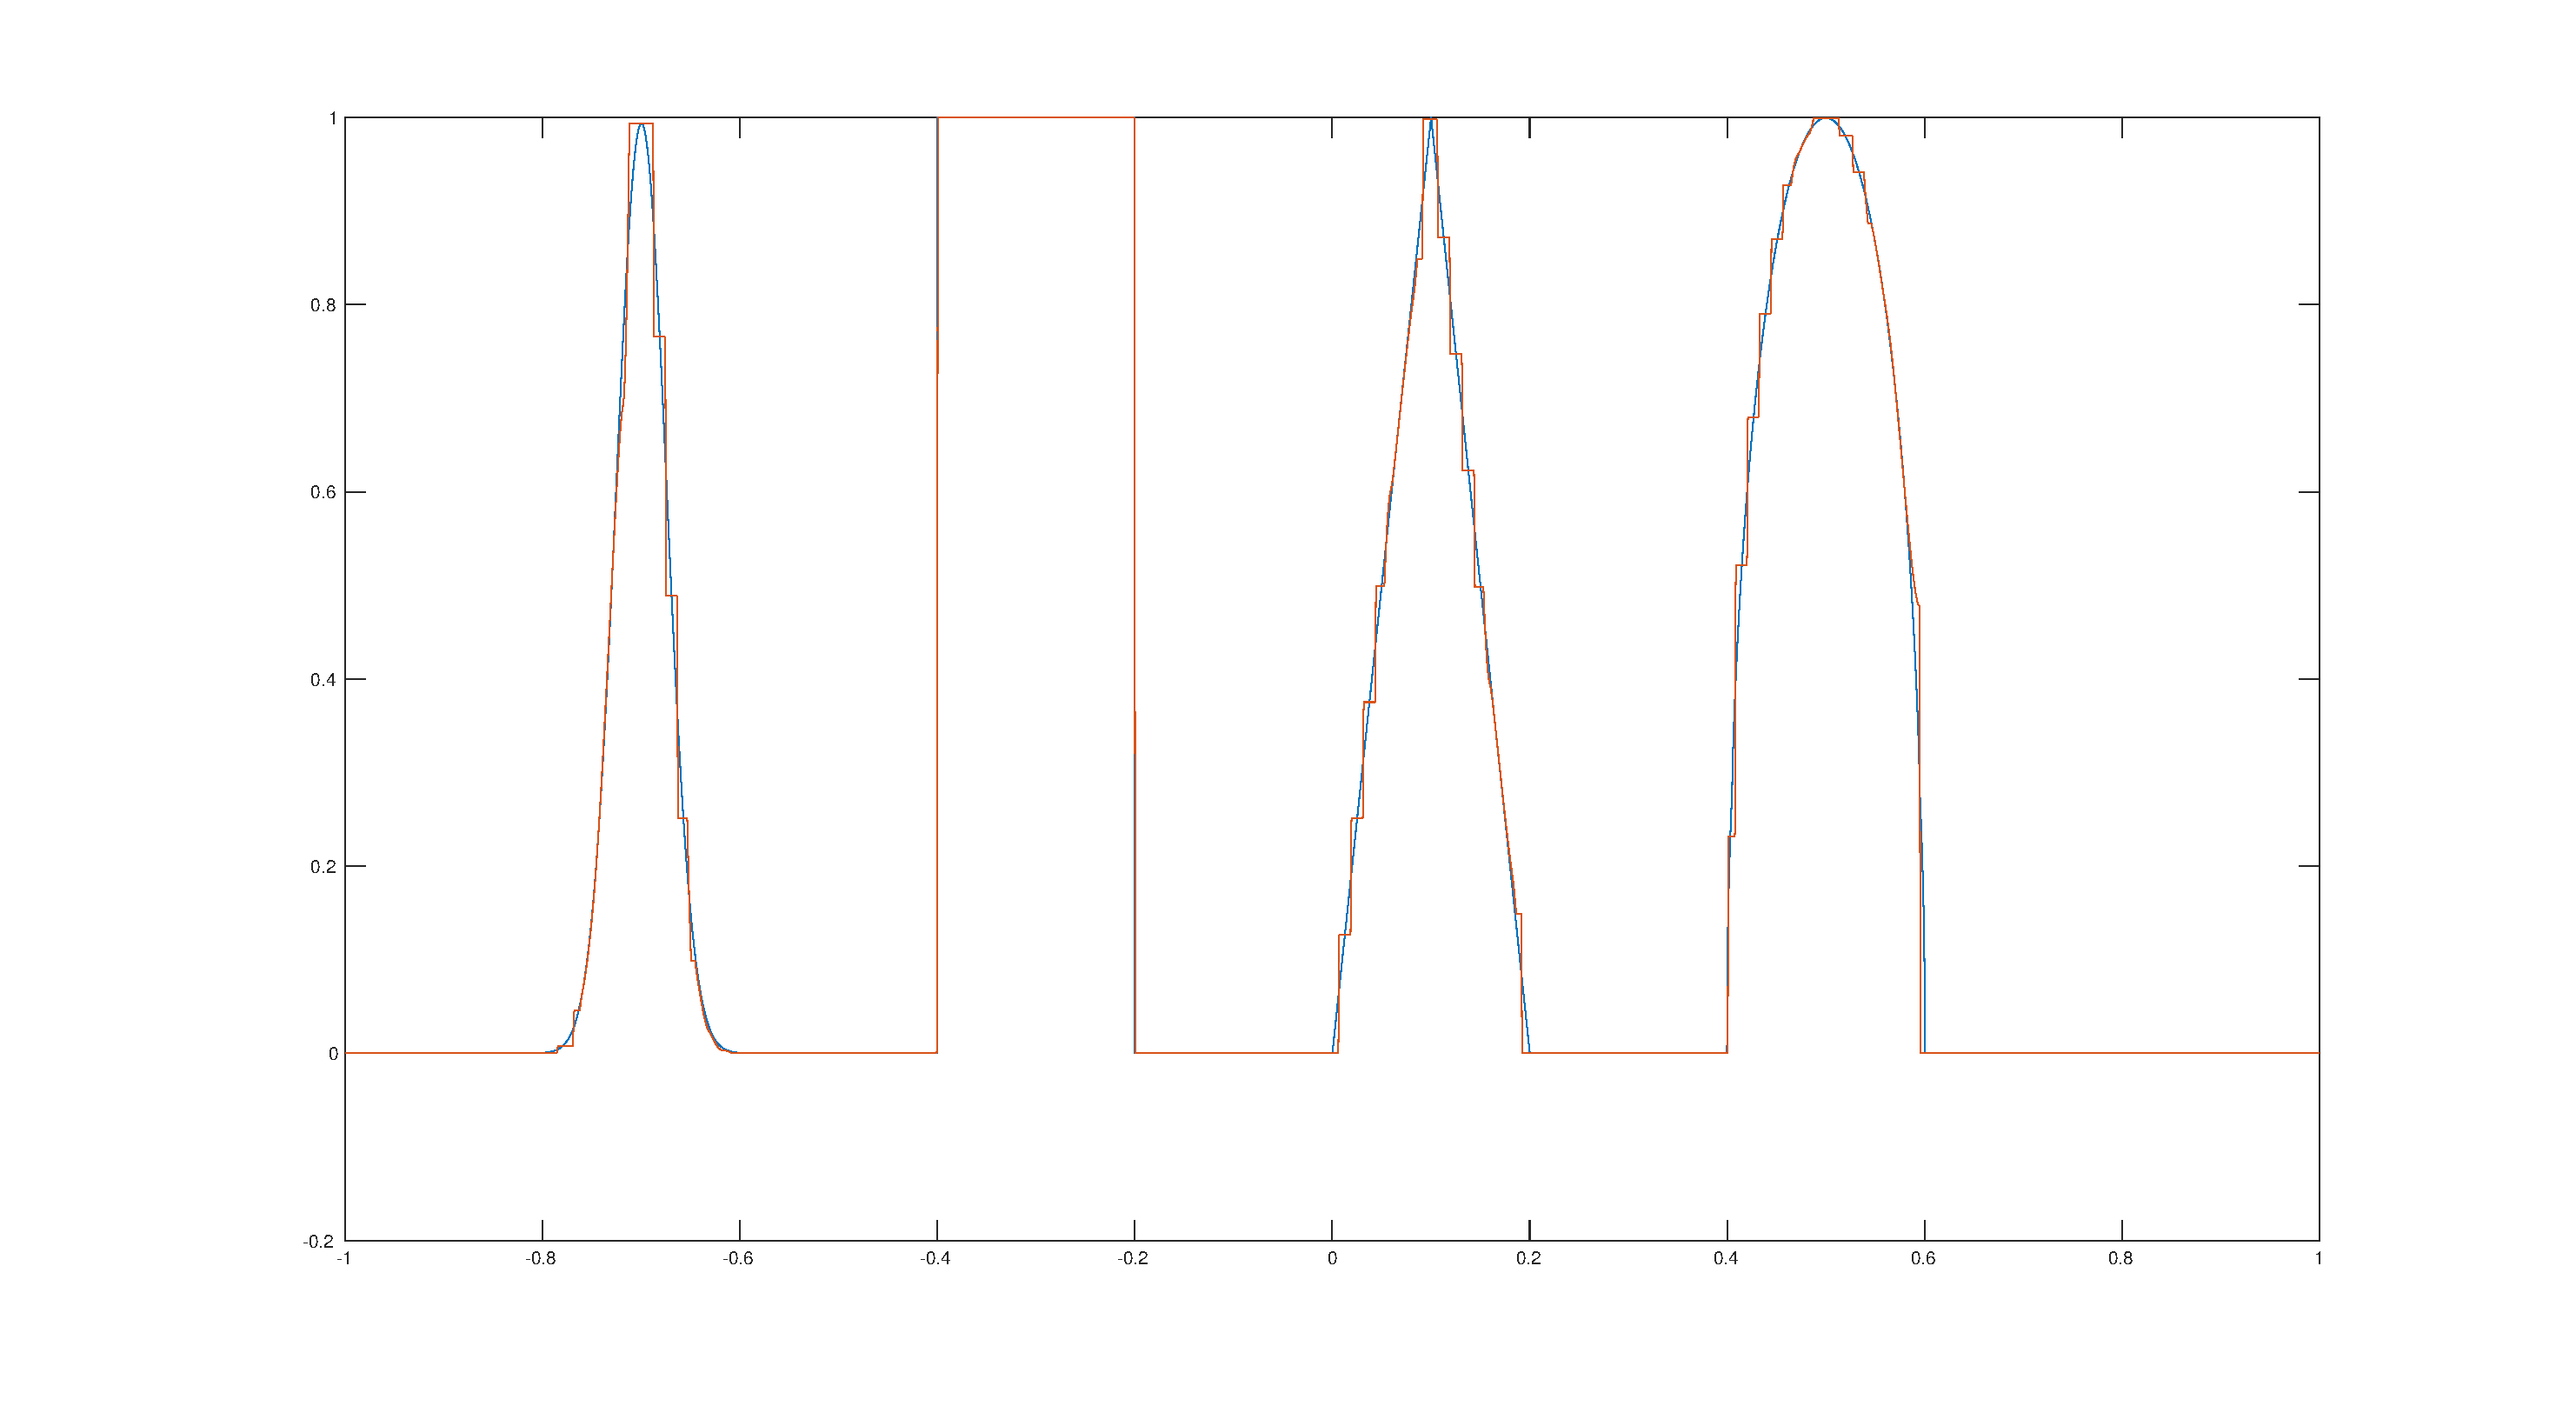
\includegraphics[width=0.45\textwidth,height=0.4\textheight]{../doc/images/advection_LF_superbee_RK3.eps}}
    \subfigure[MC]{
    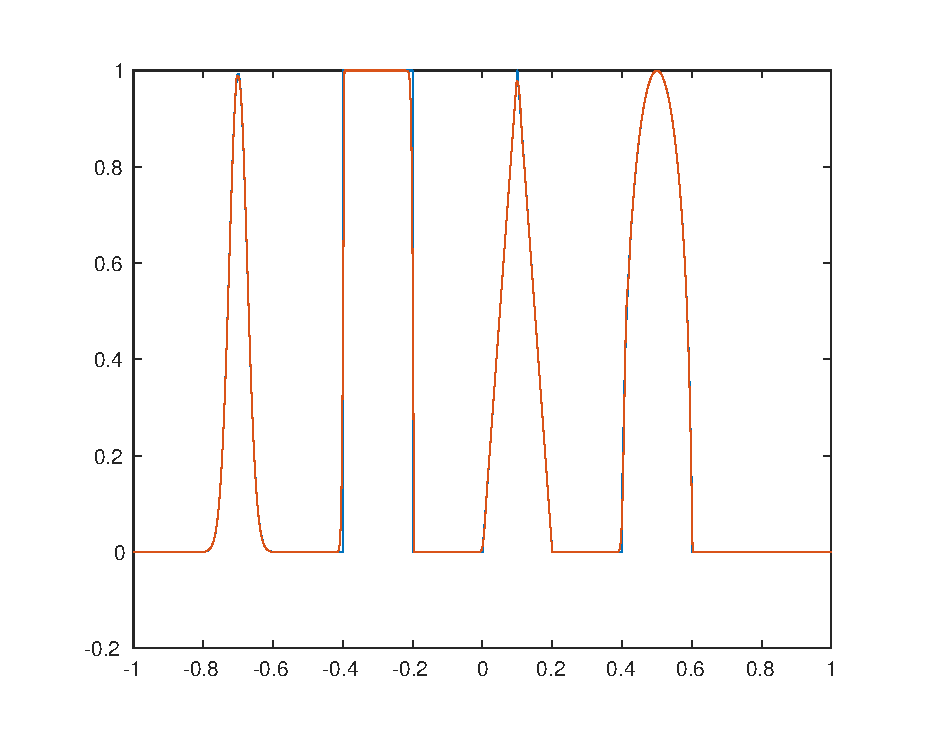
\includegraphics[width=0.45\textwidth,height=0.4\textheight]{../doc/images/advection_LF_MC_RK3.eps}}
    \subfigure[van-Leer]{
    \includegraphics[width=0.45\textwidth,height=0.4\textheight]{../doc/images/advection_LF_vanLeer_RK3.eps}}
  \end{figure}
\end{frame}
\begin{frame}
  \frametitle{各限制器比较}
  以上实验参数$N=10000,t_{end}=8,CFL=0.6$,采用的数值通量为LF通量,时
  间方向采用3阶RK格式。
  \begin{itemize}
    \item minmod: TVD,但重构效果不是很好,仍有一定耗散。
    \item superbee: 非TVD, 重构效果不是很好,会一定程度增加震荡。
    \item MC: 非TVD,数值结果尚可,但会出现负值。
    \item van-Leer: TVD,数值结果尚可。
  \end{itemize}
\end{frame}

\begin{frame}
  \frametitle{数值算例:Osher-Shu问题}
  一维Euler方程,初值为:
  \begin{equation*}
    (\rho,u,p)=\left\{
    \begin{aligned}
      &(3.857143,2.629369,10.33333),\quad &x< -4, \\
      &(1+0.2\sin (5x),0,1),\quad &x\geq -4.
    \end{aligned}
    \right.
  \end{equation*}
不加重构求解,$N=10000,t=1.8,CFL=0.6$,结果如下:
\begin{figure}[H]
  \begin{center}
    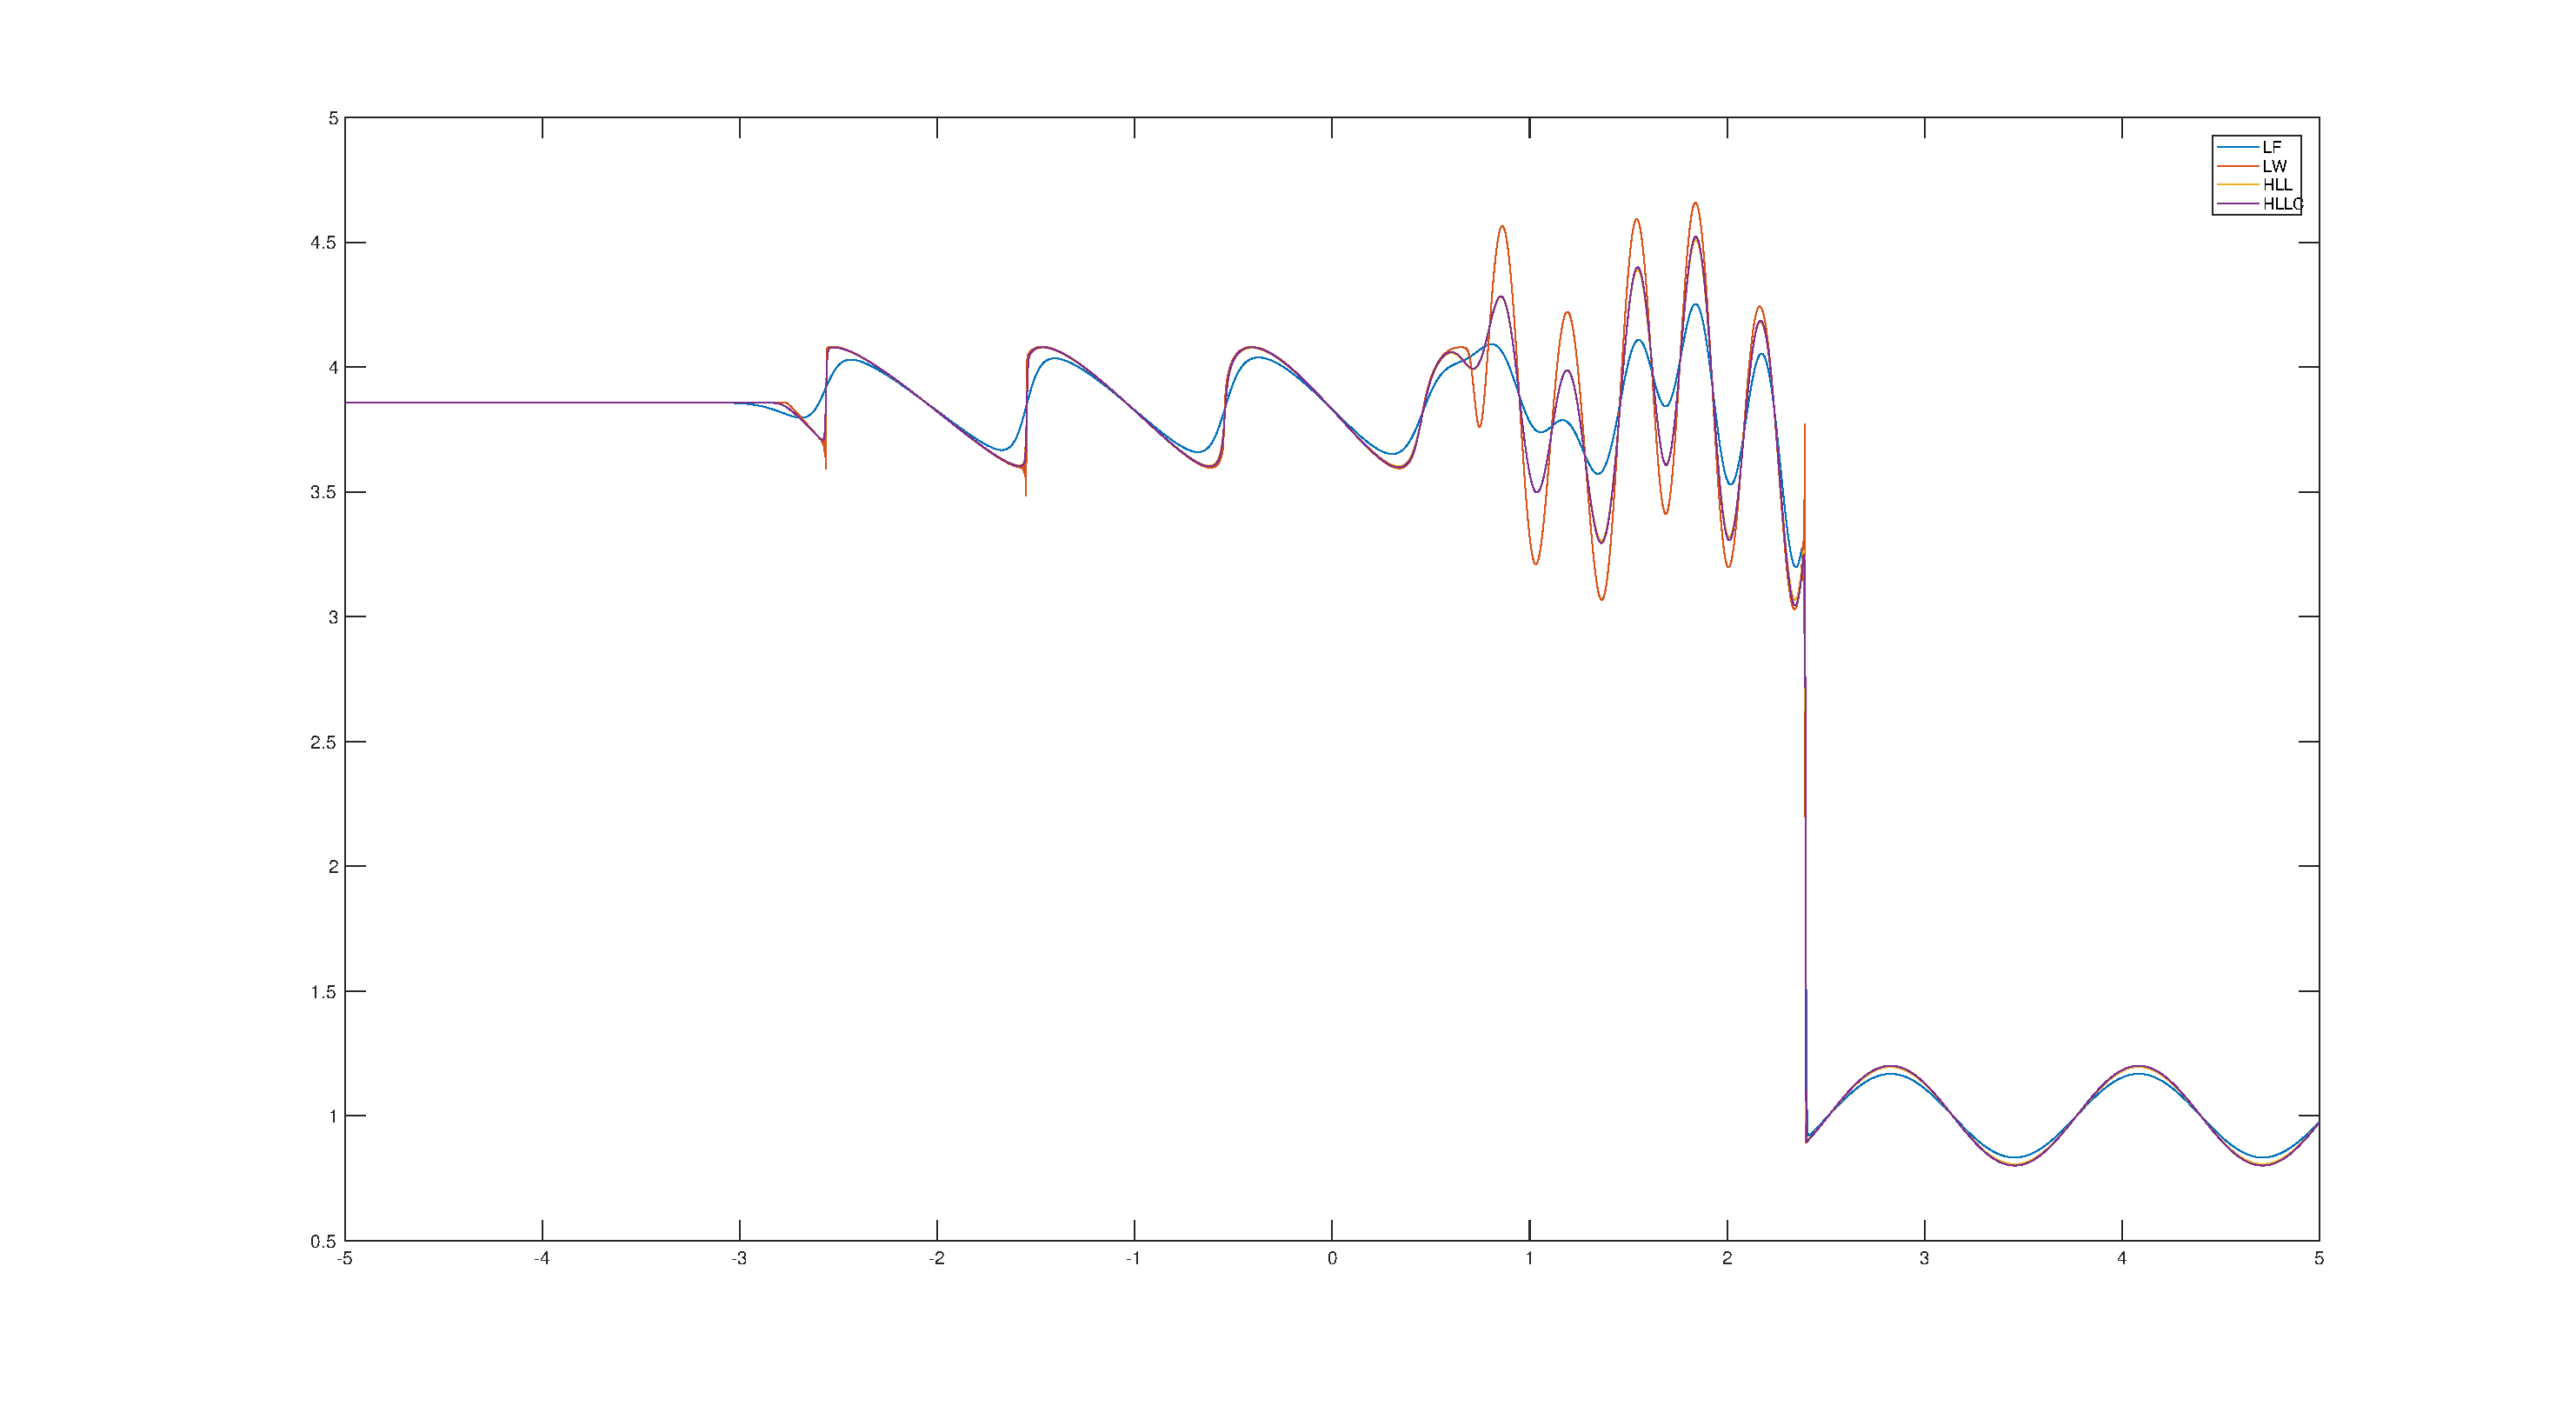
\includegraphics[width=0.9\textwidth]{../doc/images/EulerShu-Noreconstruction.eps}
  \end{center}
  \caption{Osher-Shu问题}
\end{figure}
\end{frame}

\begin{frame}
  \frametitle{各限制器比较}
  \begin{figure}[H]
    \subfigure{
    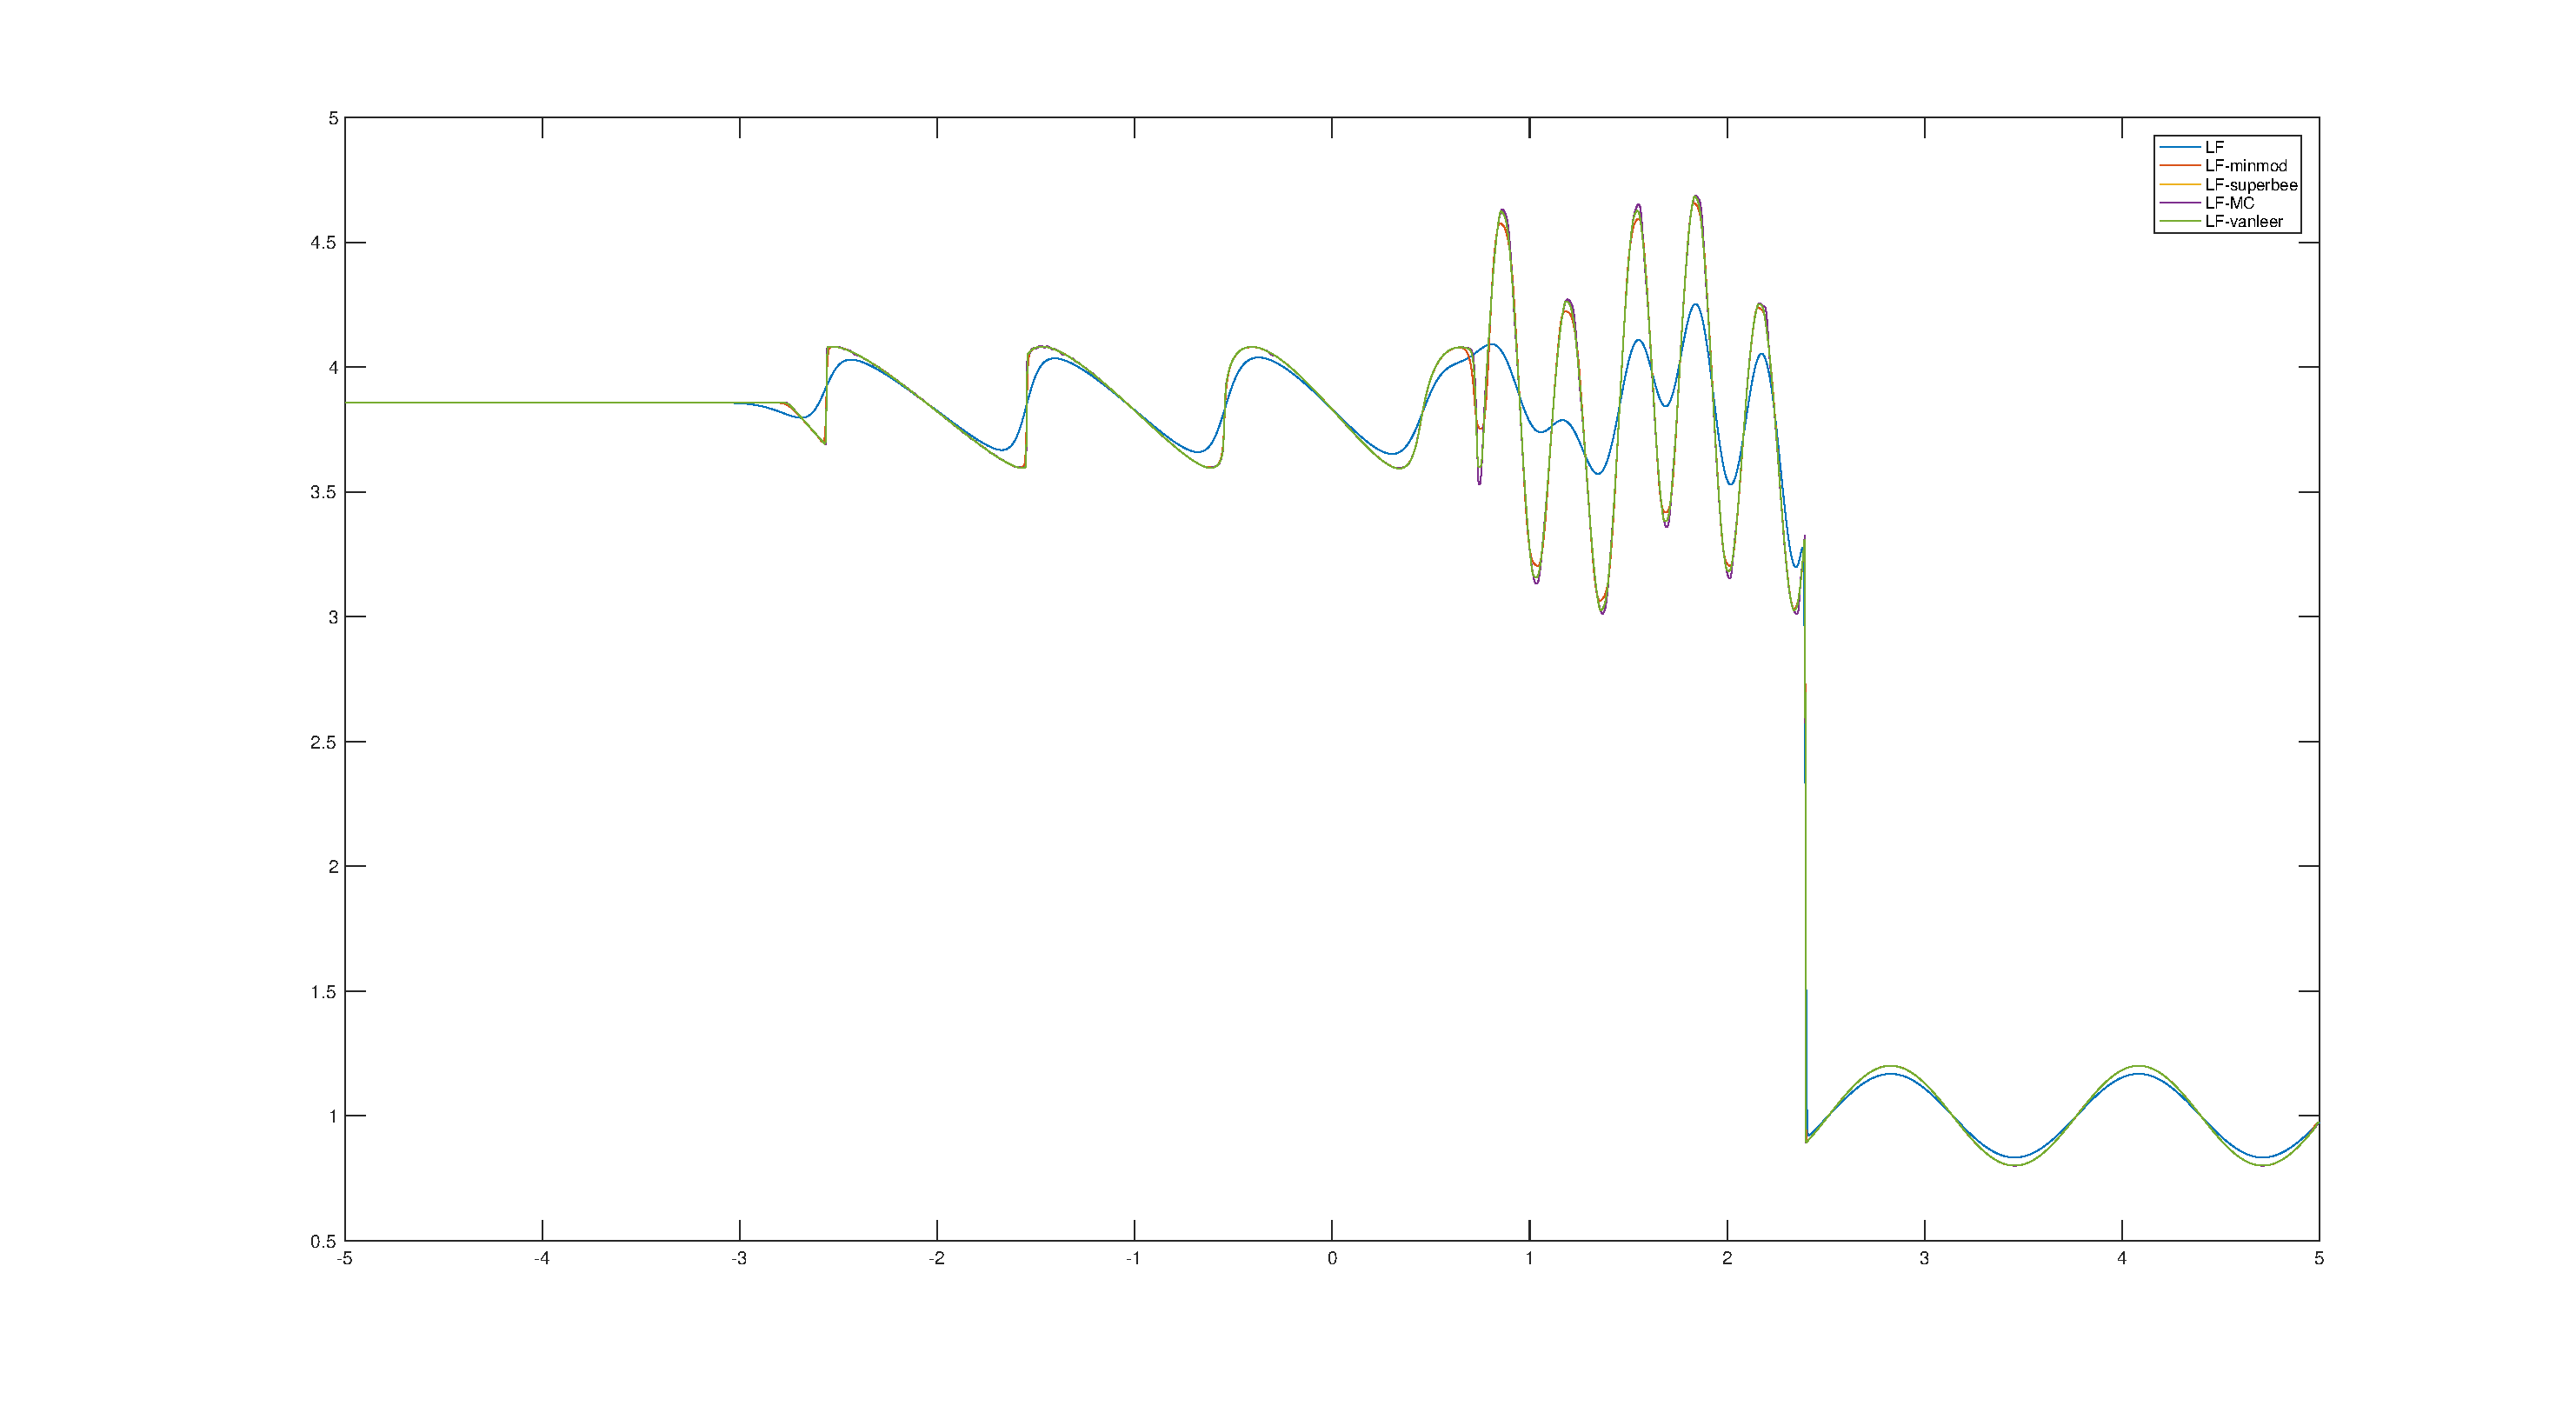
\includegraphics[width=0.45\textwidth,height=0.4\textheight]{../doc/images/EulerShu-LF.eps}}
    \subfigure{
    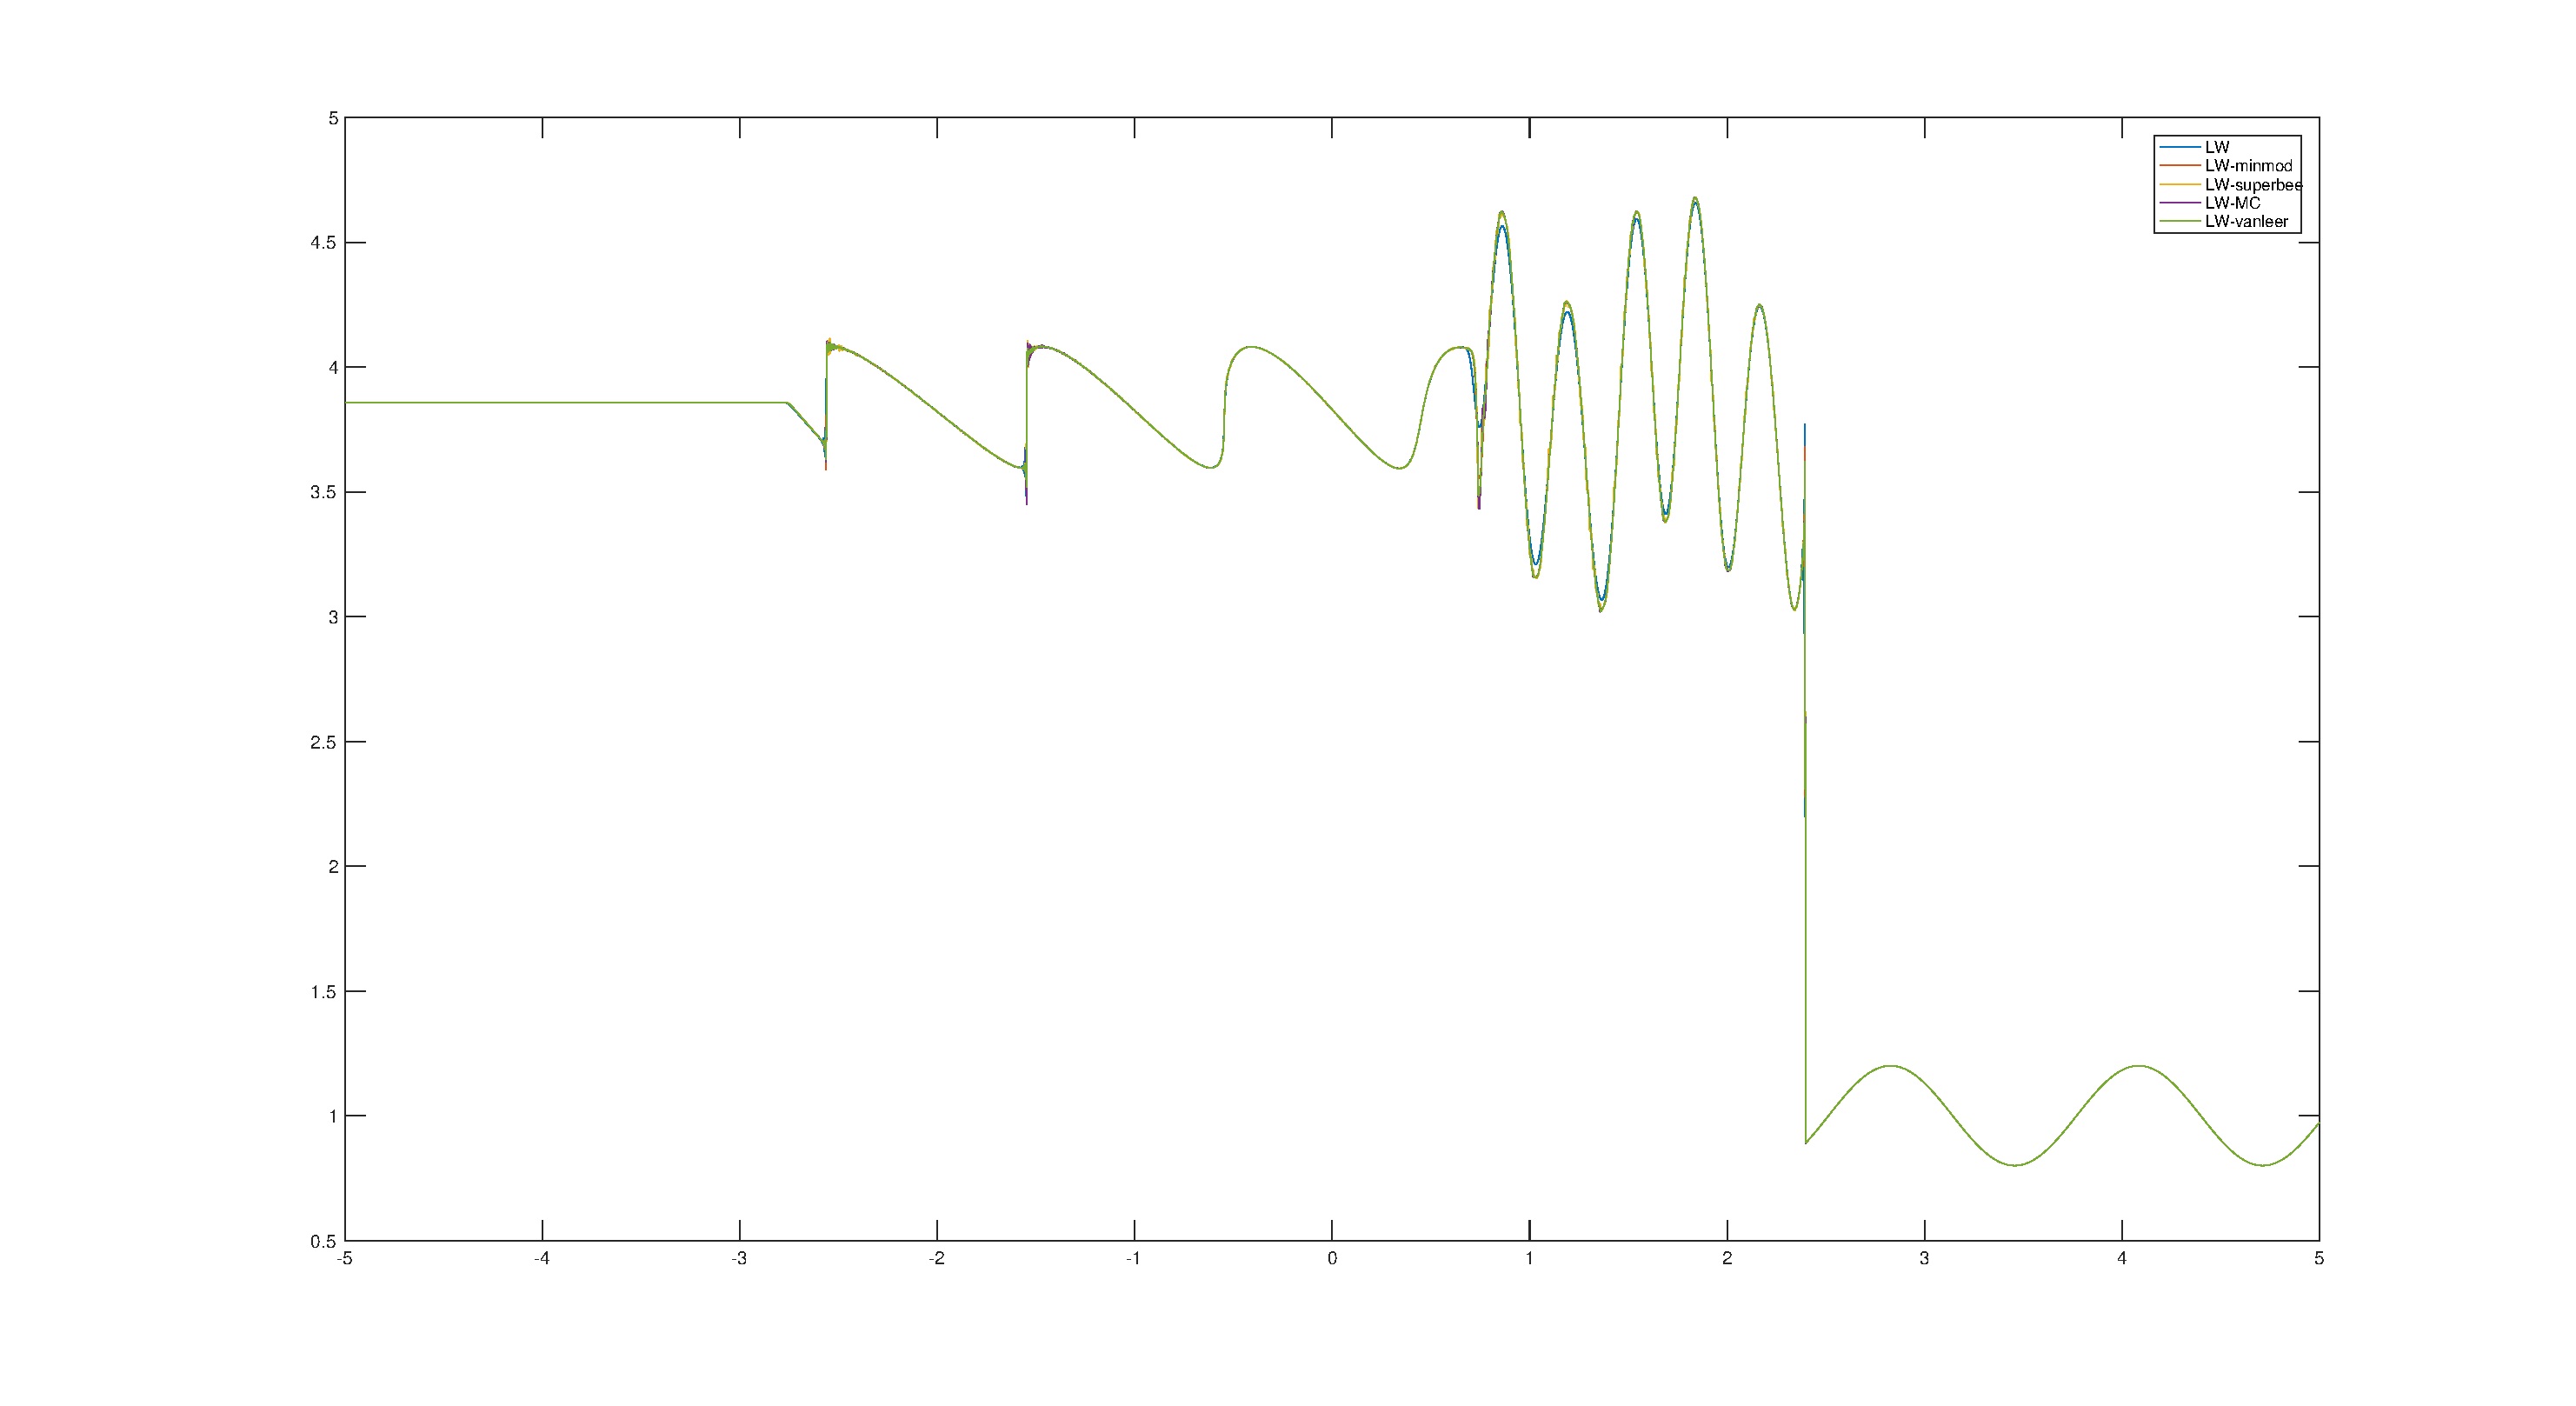
\includegraphics[width=0.45\textwidth,height=0.4\textheight]{../doc/images/EulerShu-LW.eps}}
    \subfigure{
    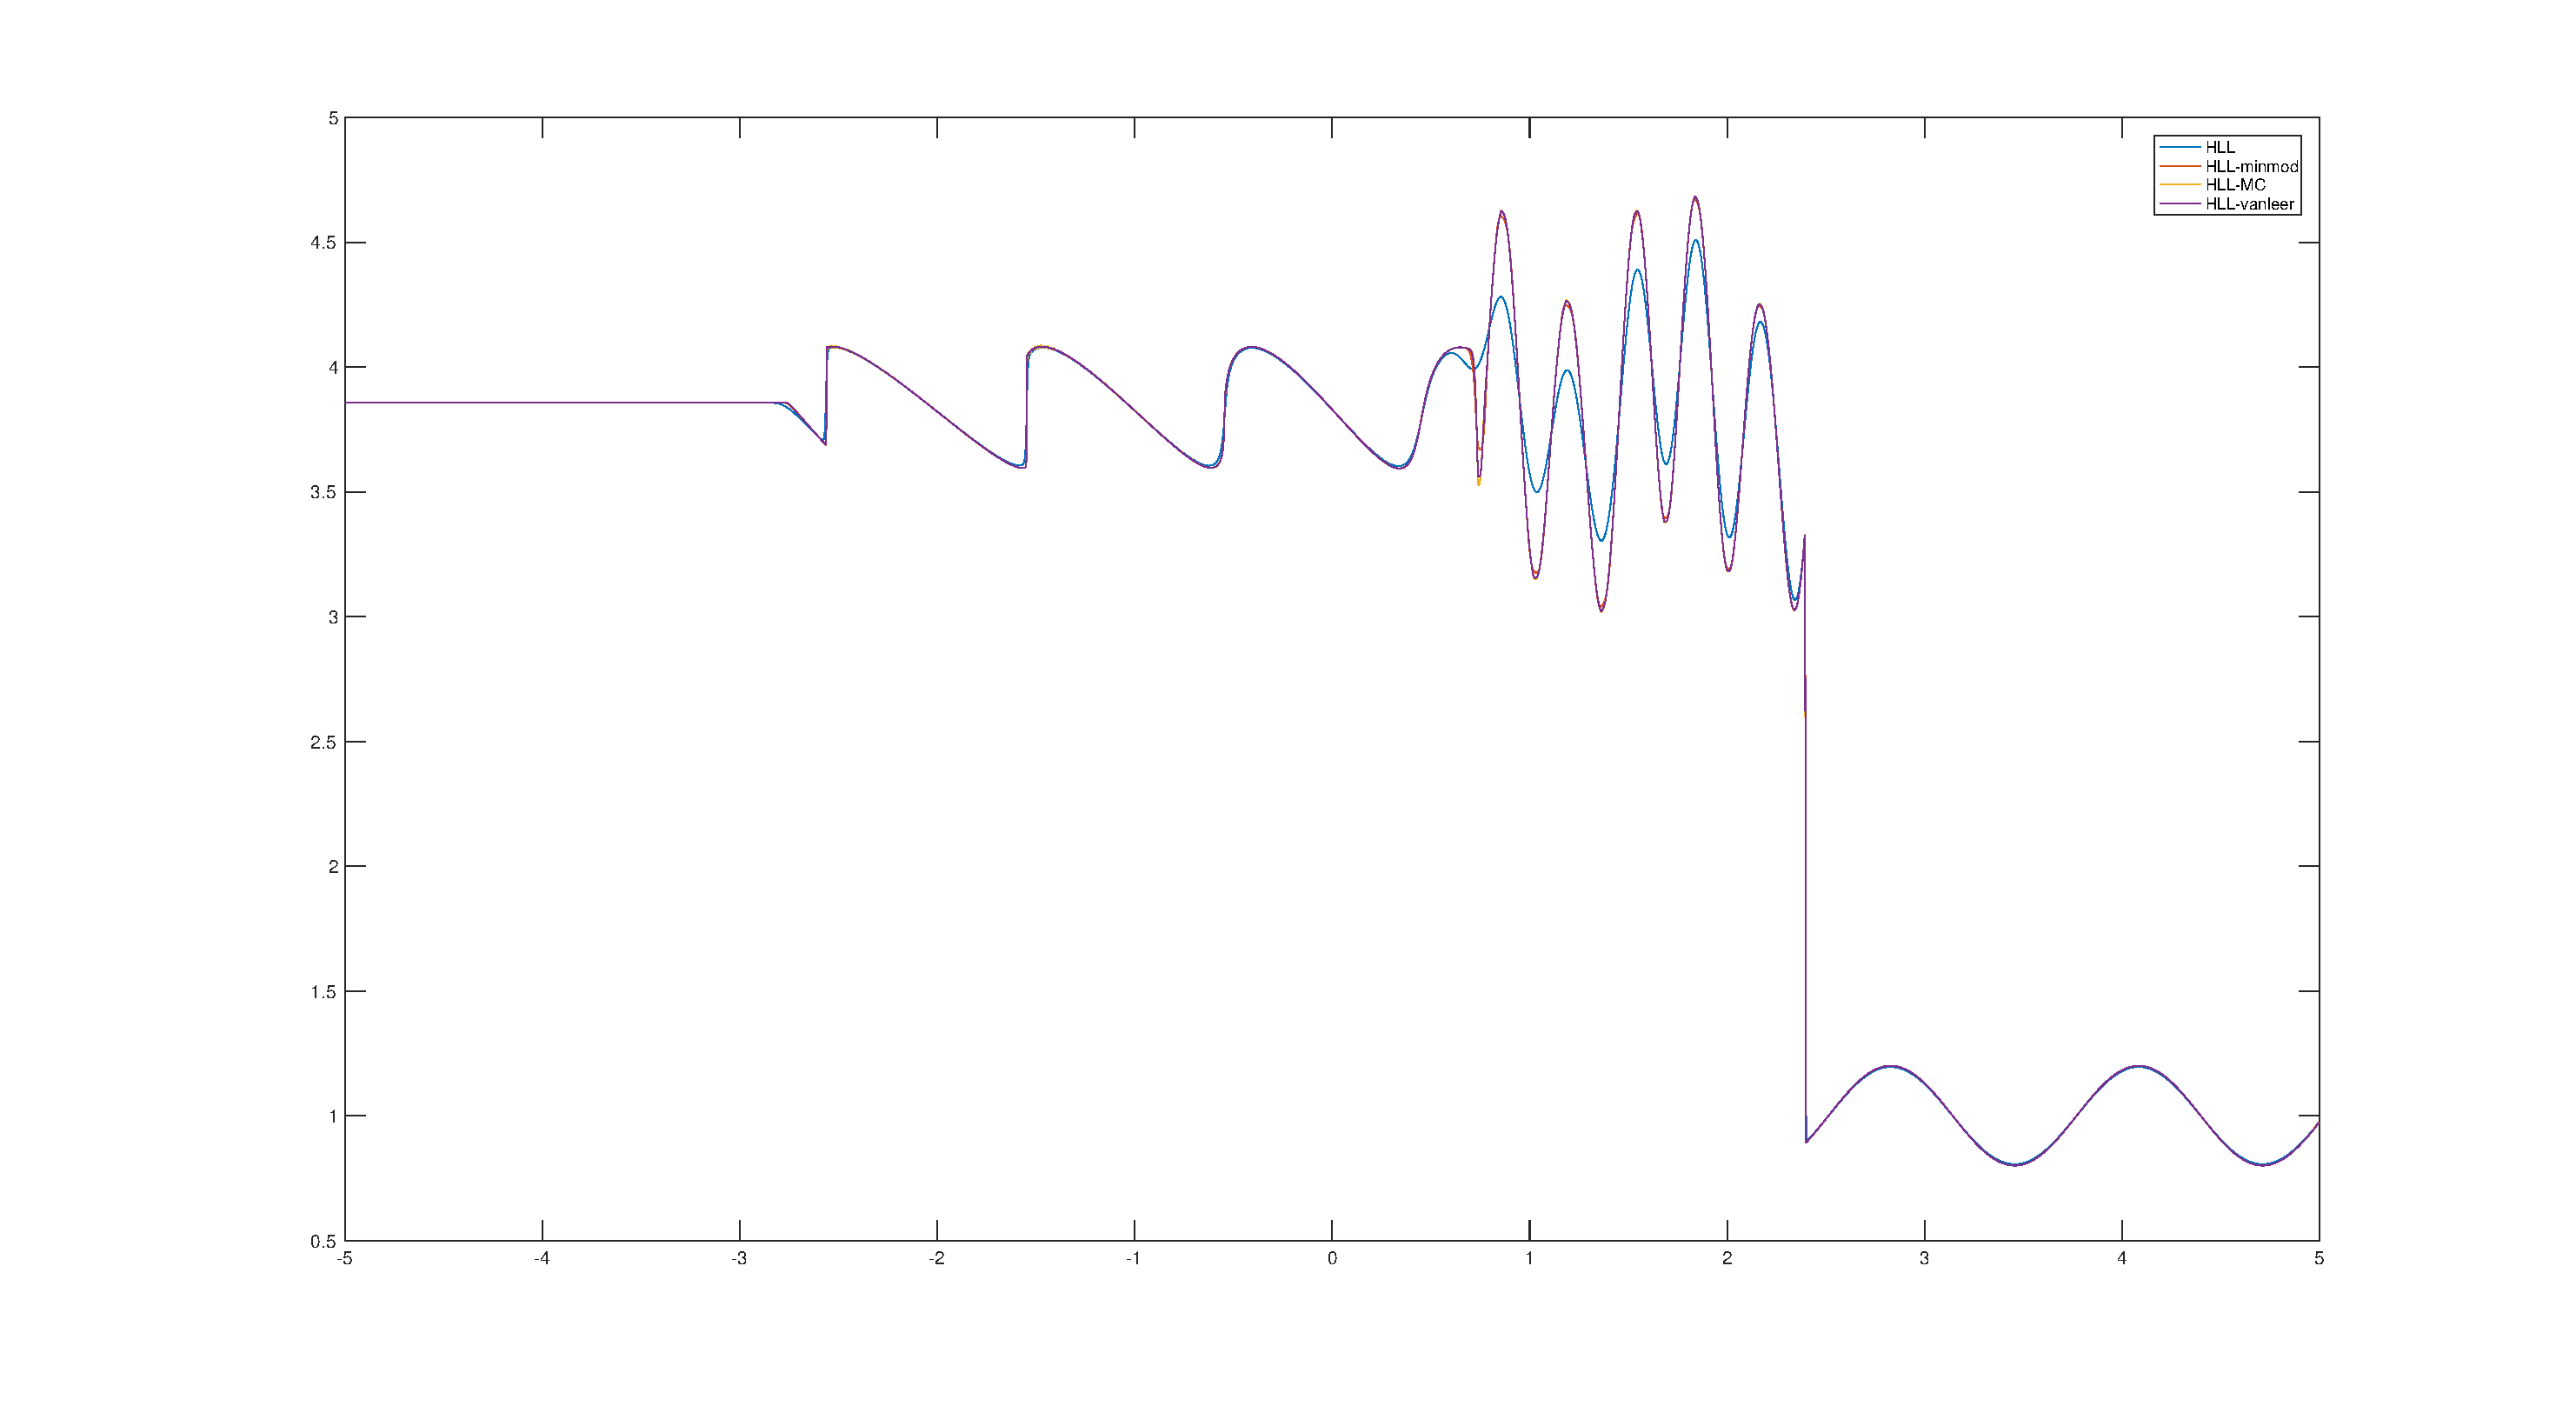
\includegraphics[width=0.45\textwidth,height=0.4\textheight]{../doc/images/EulerShu-HLL.eps}}
    \subfigure{
    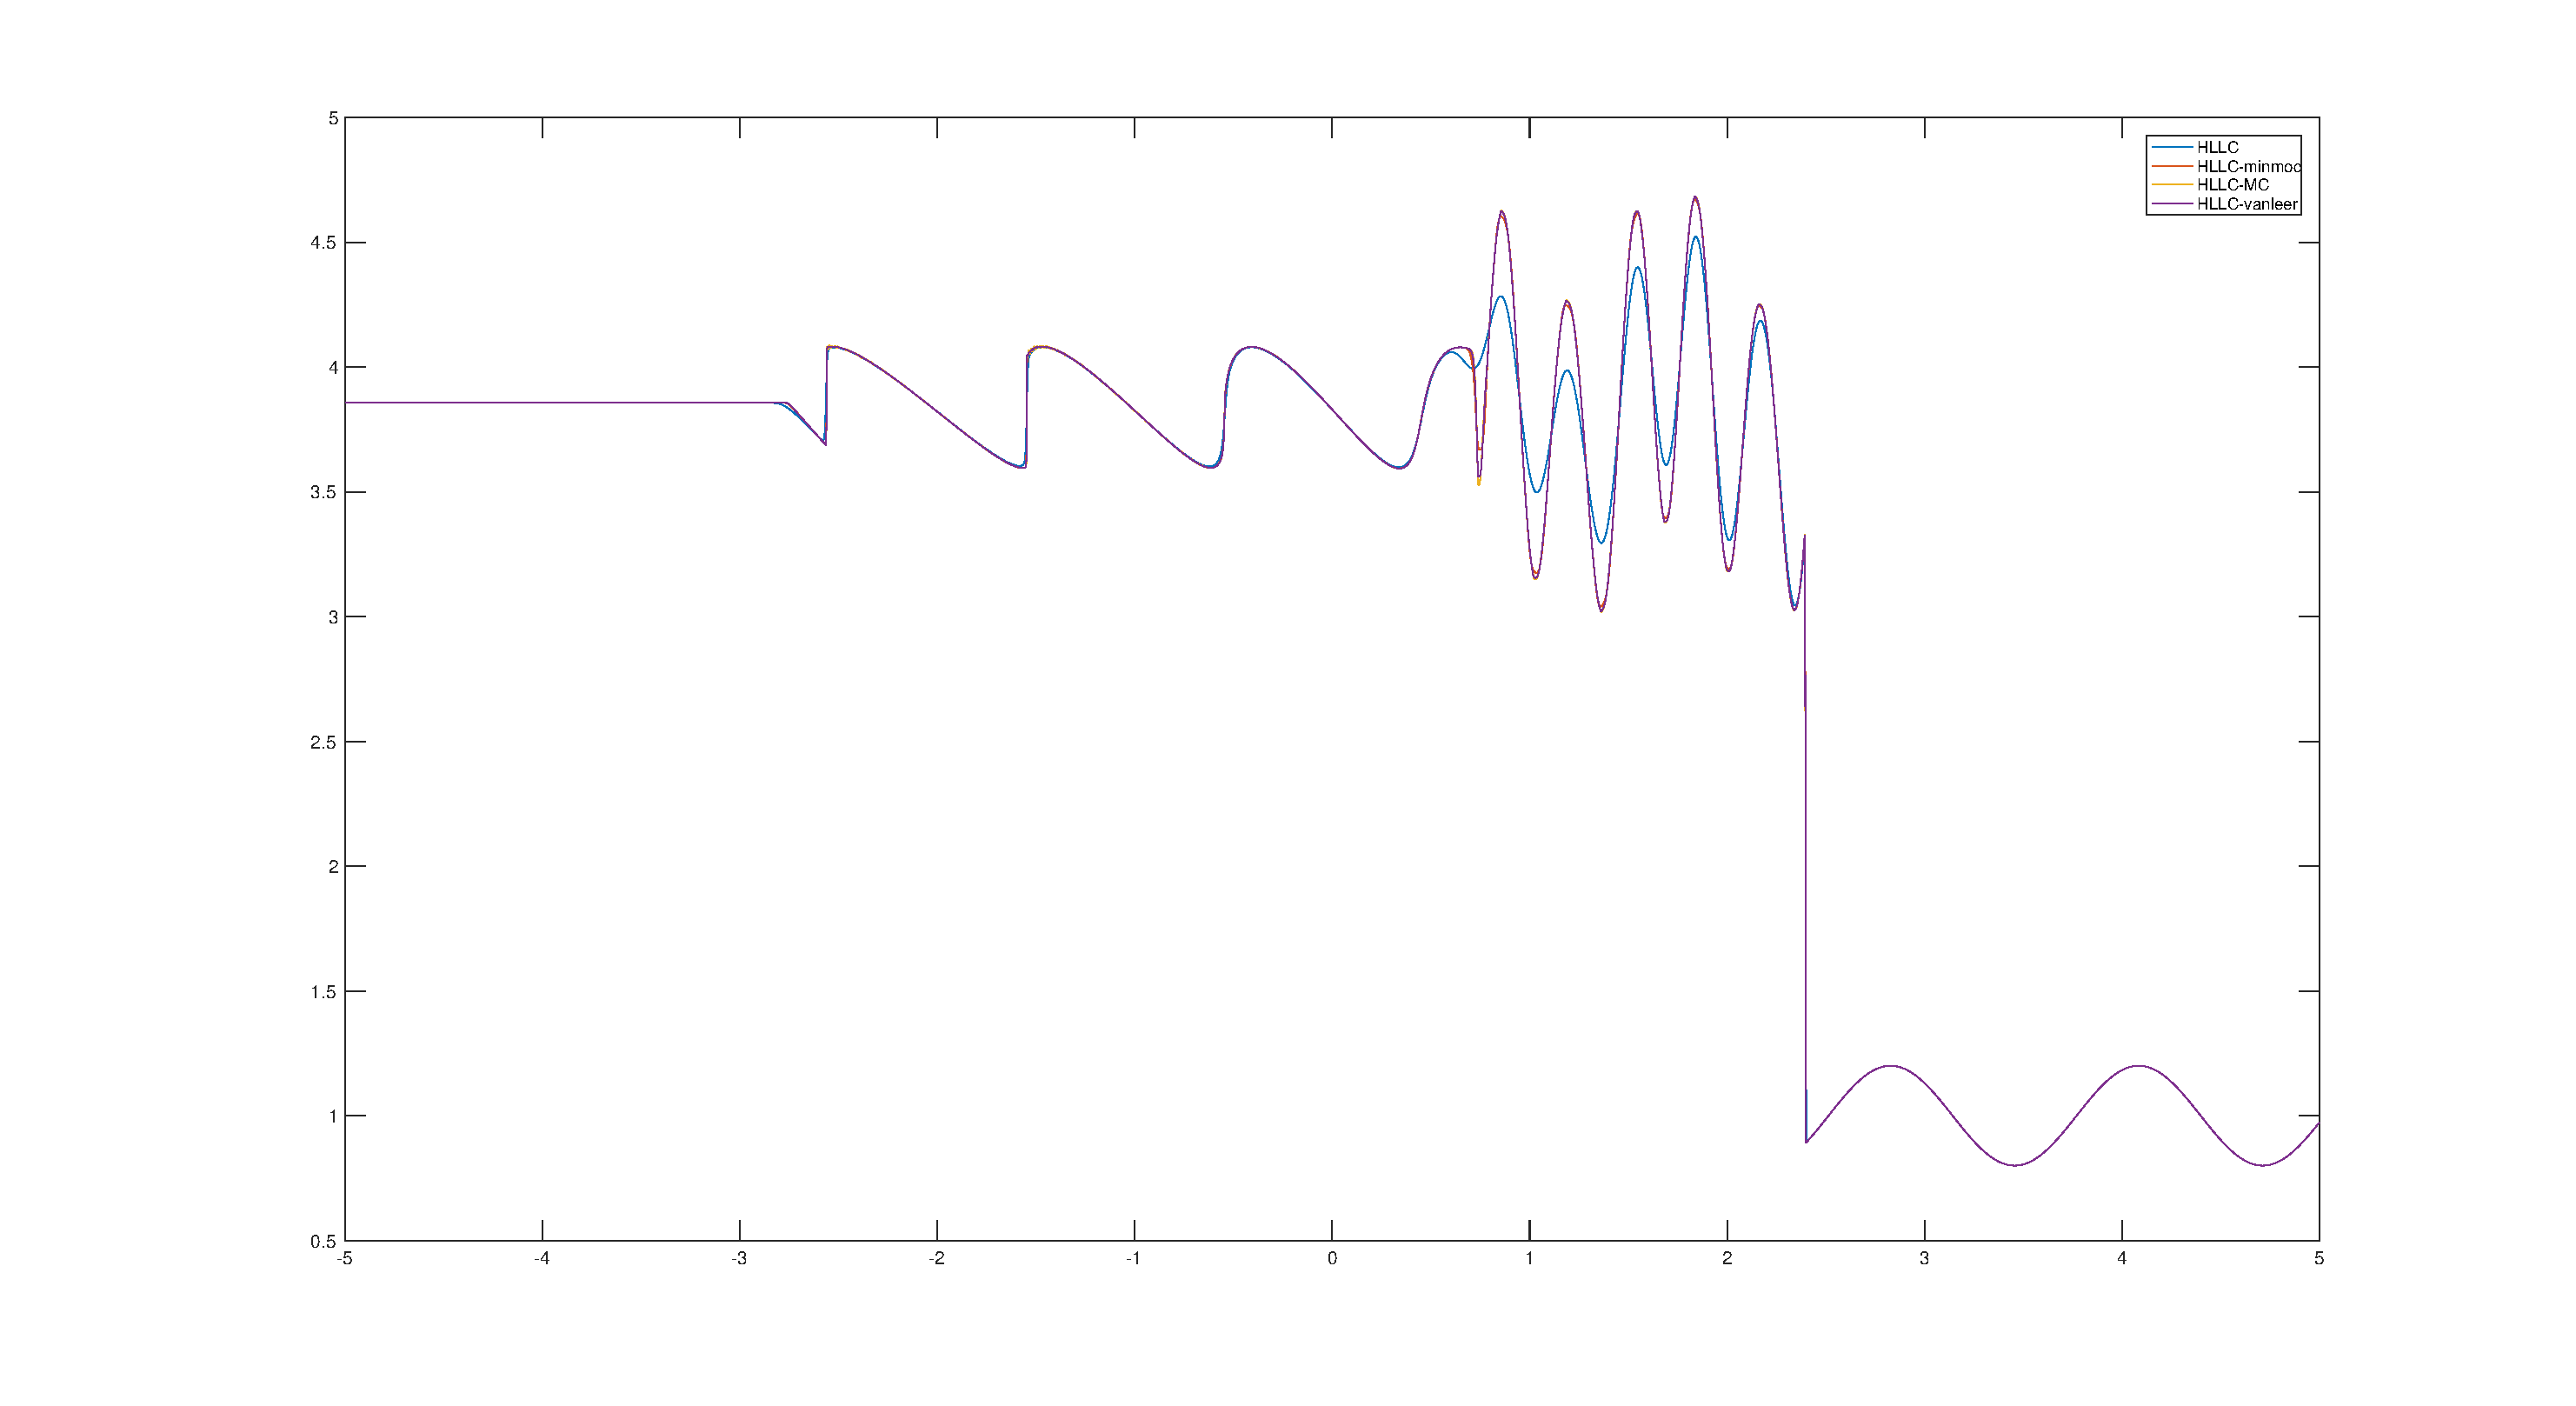
\includegraphics[width=0.45\textwidth,height=0.4\textheight]{../doc/images/EulerShu-HLLC.eps}}
  \end{figure}
\end{frame}

\begin{frame}
  \frametitle{数值算例:前台阶问题}
\begin{figure}[H]
  \begin{center}
    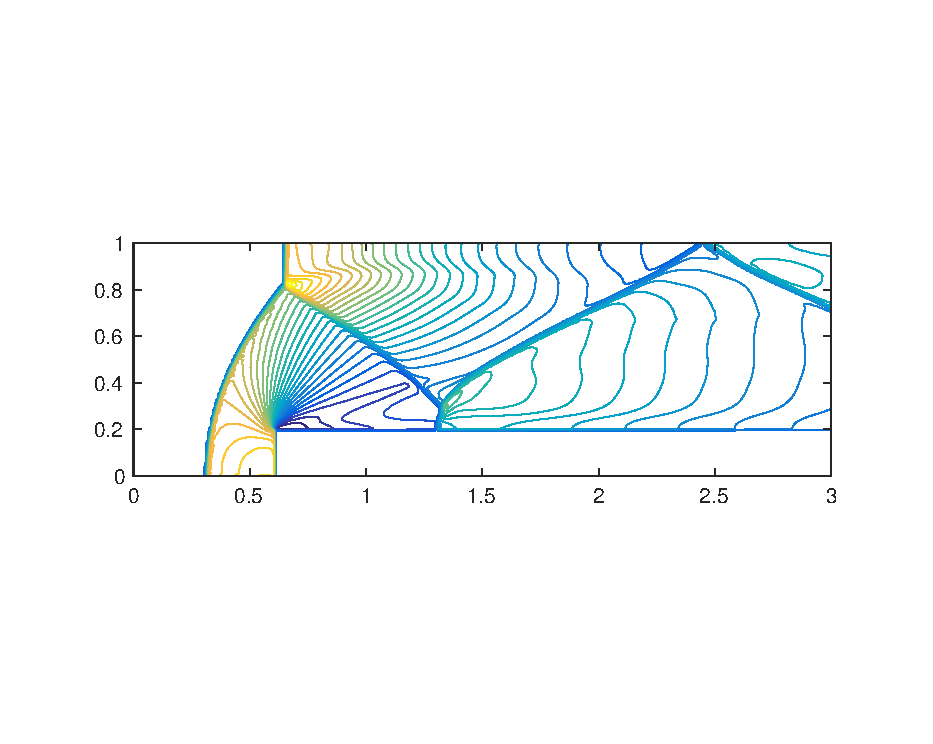
\includegraphics[width=0.9\textwidth]{../doc/images/ForwardStep-300-100-HLL-minmod.eps}
  \end{center}
  \caption{Osher-Shu问题}
\end{figure}
\end{frame}

\begin{frame}
  \frametitle{数值算例:双马赫反射问题}
\begin{figure}[H]
  \begin{center}
    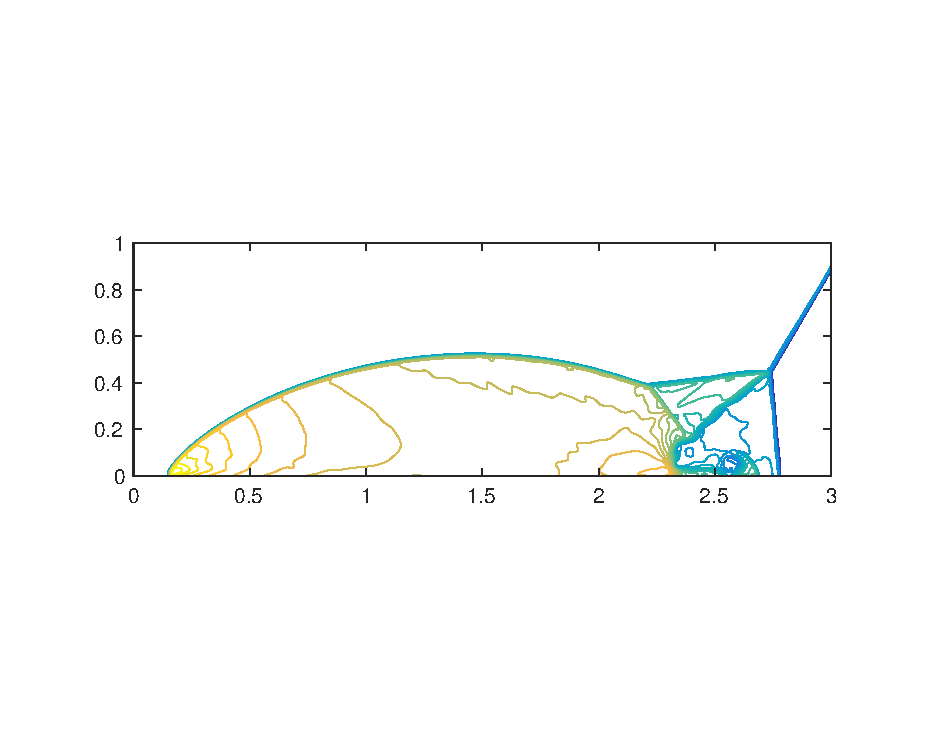
\includegraphics[width=0.9\textwidth]{../doc/images/MachReflection-960-240-MC.eps}
  \end{center}
  \caption{Osher-Shu问题}
\end{figure}
\end{frame}

\end{document}



%%% Local Variables:
%%% mode: latex
%%% TeX-master: t
%%% End:
